% ============================================================
%  Signal Credibility Score: A Multi-Phase Validation Framework
%  for Machine Learning Trading Signals
% ============================================================
\documentclass[12pt,a4paper]{article}

% PACKAGES
\usepackage[utf8]{inputenc}
\usepackage[T1]{fontenc}
\usepackage{lmodern}
\usepackage{amsmath,amssymb,amsfonts}
\usepackage{booktabs}
\usepackage{graphicx}
\graphicspath{{figures/}{uploads/figures/}}
\usepackage{hyperref}
\usepackage[margin=2.5cm]{geometry}
\usepackage{natbib}
\usepackage{caption}
\usepackage{float}
\usepackage{xcolor}

\hypersetup{colorlinks=true,linkcolor=blue,citecolor=blue,urlcolor=blue}

% TITLE
\title{%
  Signal Credibility Score: A Multi-Phase Validation Framework\\
  for Machine Learning Trading Signals%
}
\author{%
  Hamza Khan\textsuperscript{1,*} \and Alexandre Danoffre\textsuperscript{1}\\[4pt]
  \textsuperscript{1}\textit{ECE Paris, School of Engineering}\\[2pt]
  \textsuperscript{*}Corresponding author: \texttt{hamza.khan@edu.ece.fr}%
}
\date{April 2026}

\begin{document}
\maketitle

% ============================================================
\begin{abstract}
Validation protocols for machine learning trading signals remain underdeveloped, with most studies reporting in-sample metrics without rigorous out-of-sample testing across market regimes. We introduce the Signal Credibility Score (SCS), a three-phase validation framework that evaluates ML trading signals across five dimensions: temporal robustness, cross-asset generalization, inter-model consensus, stochastic stability, and distributional quality. The framework proceeds through signal discovery (Phase~A), expanding walk-forward validation (Phase~B), and frozen-model out-of-sample testing (Phase~C) with four complementary statistical tests. A performance-weighted inter-model consensus measure ($S_{\text{model}}$) conditions agreement on profitability rather than mere rank correlation, guarded by a Kish effective-$N$ threshold. Monte Carlo false discovery rate calibration (12{,}000 null trials) and oracle-based power analysis characterize the framework's operating characteristics. Applied to 12~signal groups over 27~US equities, with discovery on 2010--2013 data, a primary walk-forward stage over 2014--2022, and complementary non-overlapping OOS evaluations over 2023--2025, the framework approves 5 of 12 groups. At $\tau\geq0.70$, zero false positives are observed in 12{,}000 null trials (Clopper--Pearson 95\% CI: $[0, 0.03\%]$) while oracle injection yields 96--100\% observed detection power across the tested noise levels. Under the strict pipeline, 4 of the 5 approved groups pass Phase~B in all three OOS evaluations (2023, 2024, 2025), averaging Sharpe ratios of +0.76, +1.32, and +0.68 respectively. These results position SCS as a conservative pre-deployment validation filter rather than a performance-maximizing selector.
\end{abstract}

\medskip\noindent
\textbf{Keywords:} signal validation, false discovery rate, machine learning, systematic trading, walk-forward testing, inter-model consensus, power analysis.

\medskip\noindent
\textbf{JEL Classification:} G11, G14, C53, C58.


% ============================================================
\section{Introduction}
\label{sec:intro}

Recent work on machine learning for trading signals has demonstrated predictive power in controlled settings \citep{gu2020empirical, krauss2017deep}, but validation practices remain inconsistent. Most studies report in-sample or single-fold cross-validated metrics without rigorous multi-dimensional out-of-sample testing, leaving practitioners unable to distinguish genuine signals from artifacts of data snooping, multiple testing, and backtest multiplicity \citep{harvey2015backtesting, bailey2014deflated}.

We propose the Signal Credibility Score (SCS), a three-phase composite metric that evaluates ML trading signals across temporal robustness, cross-asset generalization, inter-model consensus, stochastic stability, and distributional quality. Each dimension addresses a distinct failure mode: a signal may work in one time period but not another ($S_{\text{time}}$), on some assets but not broadly ($S_{\text{asset}}$), with one model type but not across architectures ($S_{\text{model}}$), or may be sensitive to random initialization ($S_{\text{seed}}$) or produce pathological trade distributions ($S_{\text{dist}}$). The inter-model consensus component uses a performance-weighted Spearman formulation that assigns zero weight to conditions where no model is profitable, guarded by a Kish effective-$N$ threshold \citep{kish1965survey} to prevent concentration bias.

The framework's contributions are:

\begin{enumerate}
  \item \textbf{Multi-dimensional signal validation.} SCS aggregates five normalized sub-scores into a composite gate, with hard pre-filters (negative mean Sharpe, insufficient positive ratio) and a transparent approval threshold. Three temporally separated phases---discovery, walk-forward, and frozen-model OOS testing---prevent information leakage.
  \item \textbf{Performance-weighted inter-model consensus ($S_{\text{model}}$).} Rather than measuring rank correlation unconditionally, the consensus component conditions on profitability: models must agree specifically on \emph{profitable} conditions. A Kish effective-$N$ guard prevents concentrated conditions from dominating the estimate.
  \item \textbf{Multi-window out-of-sample testing.} Approved signals are evaluated across three non-overlapping OOS years---2023, 2024, and 2025---using expanding walk-forward windows, revealing regime-dependent variation that single-year testing obscures.
  \item \textbf{FDR calibration and power analysis.} The full Phase~A pipeline is run under 1{,}000 seeds of 100\% label corruption (12{,}000 group-level null trials) to calibrate empirical false positive rates. Oracle signal injection across 50 seeds at 10 noise levels characterizes detection power. At $\tau=0.70$, zero false positives are observed in 12{,}000 null trials while observed oracle power ranges from 96\% to 100\% across the tested noise levels.
\end{enumerate}

Beyond these core contributions, we conduct threshold sensitivity analysis, progressive label corruption as a negative control, comparison with standard selection strategies, and oracle feature injection---stress tests that collectively establish the framework's operating characteristics.

The paper proceeds as follows. Section~\ref{sec:literature} situates the contribution in the broader literature. Section~\ref{sec:methodology} describes the SCS framework. Section~\ref{sec:data} presents the data and experimental setup. Section~\ref{sec:results} reports empirical results including multi-window OOS performance. Section~\ref{sec:experiments} details the validation experiments. Section~\ref{sec:discussion} discusses implications and limitations. Section~\ref{sec:conclusion} concludes.


% ============================================================
\section{Related Work}
\label{sec:literature}

\textbf{Multiple testing and false discoveries.} The problem of inflated significance in empirical finance is well established. \citet{harvey2015backtesting} propose a minimum $t$-statistic of 3.0 for new factor discoveries; \citet{harvey2016cross} formalize this and show most published factors fail to survive it. \citet{bailey2014deflated} develop the Deflated Sharpe Ratio, correcting observed Sharpe ratios for the number of configurations tested. \citet{white2000reality} introduce the Reality Check bootstrap for detecting data-snooped outperformance. \citet{cawley2010overfitting} show that even model selection criteria can overfit, motivating fixed-parameter designs. The SCS framework integrates DSR at Phase~C, uses fixed hyperparameters, and provides formal false positive rate calibration via Monte Carlo simulation.

\textbf{Walk-forward testing and cross-validation.} \citet{pardo2008evaluation} formalize walk-forward analysis; \citet{lopez2018advances} (ch.~7) introduces purged $k$-fold cross-validation to prevent leakage from overlapping labels. \citet{bailey2017probability} extend this with combinatorial purged cross-validation (CPCV) for estimating the probability of backtest overfitting. Our expanding-window walk-forward design with 6 annual folds and dual cost scenarios operationalizes these ideas; the multi-window OOS extension evaluates signals across three distinct market regimes rather than a single test period.

\textbf{Performance measurement.} The Sharpe ratio \citep{sharpe1994sharpe} remains the standard risk-adjusted metric. \citet{ledoit2008robust} provide a HAC-robust comparison test that we apply at Phase~C. A key insight from prior work is that single-year track records have inherently low power; our multi-window design addresses this limitation empirically.

\textbf{ML signal decay and the factor replication crisis.} \citet{gu2020empirical} show gradient-boosted trees capture cross-sectional predictability; \citet{krauss2017deep} and \citet{fischer2018deep} document ML-based returns that decay over time. On the skeptical side, \citet{mclean2016does} find $\sim$32\% post-publication factor decay, \citet{harvey2020false} estimate over half of published factors are false, \citet{chen2022open} show many do not survive modern standards, and \citet{chordia2020anomalies} find most anomalies vanish after transaction costs. \citet{arnott2019backtesting} document systematic backtesting bias. These concerns motivate the SCS emphasis on pre-specified validation with go/no-go gates, and underscore the need for formal FDR calibration of the approval threshold.


% ============================================================
\section{Methodology}
\label{sec:methodology}

We adopt a three-phase SCS pipeline with five sub-scores per phase. This section describes the full pipeline.

\subsection{Framework Overview}

The pipeline proceeds through three temporally separated phases:

\begin{itemize}
  \item \textbf{Phase A --- Signal Discovery} (2010--2013): Exhaustive search over $H \times L \times M \times S \times T$ configurations, where $H$ = horizons, $L$ = labeling strategies, $M$ = model types, $S$ = random seeds, $T$ = sub-periods. Computes SCS-A for each signal group $(H, L)$.
  \item \textbf{Phase B --- Walk-Forward Validation} (2014--2022): Expanding-window walk-forward on SCS-A-approved signals. Tests under baseline and stress transaction costs. Computes SCS-B.
  \item \textbf{Phase C --- Primary Out-of-Sample Evaluation} (2023): Frozen models from Phase~B applied to unseen data. Full portfolio backtest with statistical significance testing. Section~\ref{sec:multiwindow} later extends this evaluation to 2024 and 2025 for complementary regime analysis.
\end{itemize}

Each signal group is a $(H, L)$ pair evaluated across all model types, so that the inter-model consensus component $S_{\text{model}}$ can assess cross-model agreement.

\subsection{Labeling}

Two labeling strategies generate prediction targets:

\begin{itemize}
  \item \textbf{Directional binary}: $y_t = \mathbf{1}[r_t(H) > 0]$, where $r_t(H) = \text{Close}(t+H)/\text{Open}(t+1) - 1$.
  \item \textbf{Ternary volatility-adaptive}: With rolling volatility $\sigma_t$ over $W$ days and threshold multiplier $\theta$:
    \begin{equation}
      y_t = \begin{cases}
        2 \text{ (bullish)} & \text{if } r_t(H) > +\theta\sigma_t \\
        0 \text{ (bearish)} & \text{if } r_t(H) < -\theta\sigma_t \\
        1 \text{ (neutral)} & \text{otherwise}
      \end{cases}
    \end{equation}
\end{itemize}

With $\theta=0.5$, the neutral zone captures roughly 10--15\% of observations, filtering out low-conviction periods from the training objective.

\subsection{Purged Temporal Split with Embargo}

An embargo gap of $E \geq H$ trading days separates the last training sample from the first test sample. With a maximum label horizon of $H=20$ days, we set $E=25$, adding a 5-day buffer for calendar effects. This ensures strict temporal separation; an automated leakage test in the test suite verifies the constraint (see the code repository).

\subsection{SCS-A: Signal Discovery Score}

The discovery-phase score aggregates five normalized components:

\begin{equation}
  \text{SCS-A} = \sum_{k=1}^{5} w_k \cdot S_k
\end{equation}

with $S_k \in [0, 1]$ and $\sum w_k = 1$. Four components measure distinct robustness dimensions: $S_{\text{time}}$ (temporal robustness, 25\%), $S_{\text{asset}}$ (cross-asset generalization, 25\%), $S_{\text{seed}}$ (stochastic stability, 15\%), and $S_{\text{dist}}$ (trade-level distributional quality, 10\%). Their functional forms are detailed in Appendix~\ref{app:scs_a}. The fifth component measures inter-model consensus:

$S_{\text{model}}$ (25\%): \textbf{Performance-weighted inter-model rank consensus.} For each (ticker, period) condition $c$, the weight is $w_c = \max(\max_i \text{SR}_{i,c}, 0)$, assigning zero weight to conditions where no model is profitable. The consensus score is $\max(\bar{\rho}_w, 0)$, where $\bar{\rho}_w$ is the mean pairwise weighted Spearman correlation across model pairs. A Kish effective-$N$ guard \citep{kish1965survey} ($N_{\text{eff}} \geq 5$) prevents concentrated conditions from dominating the estimate; if the guard triggers, $S_{\text{model}} = 0$. The threshold $N_{\text{eff}}=5$ ensures that the weighted correlation draws on at least five effectively independent conditions---a common minimum for rank-correlation reliability \citep{kish1965survey}; in our setup with $3 \times 3 = 9$ to $3 \times 27 = 81$ raw conditions, the guard triggers only when one or two conditions carry the vast majority of the weight. A simpler alternative---counting statistically significant pairwise correlations without conditioning on profitability---can inflate consensus when models agree on losing trades; the performance-weighted formulation avoids this. The design is detailed in Appendix~\ref{app:scs_a}.

\textbf{Hard gates:} Groups with mean Sharpe $< 0$, positive ratio $< 50\%$, or fewer than 8 trades per bucket are rejected with SCS-A\,=\,0.

\textbf{Approval:} SCS-A $\geq 0.70 \Rightarrow$ PHASE\_B\_APPROVED.

\subsection{SCS-B: Walk-Forward Validation Score}

Phase~B scores each approved signal under expanding walk-forward conditions:

\begin{equation}
  \text{SCS-B} = \sum_{k=1}^{5} w_k \cdot S_k^{(B)}
\end{equation}

The five components measure walk-forward temporal robustness ($S_{\text{time}}^{(B)}$, 25\%), cross-asset persistence ($S_{\text{asset}}^{(B)}$, 25\%), cost tolerance ($S_{\text{cost}}$, 20\%---the ratio of stress-cost Sharpe to baseline-cost Sharpe), structural stability ($S_{\text{struct}}$, 15\%---mean pairwise correlation of per-asset Sharpe vectors across windows), and economic coherence ($S_{\text{eco}}$, 15\%---plausibility of trade frequency for the given horizon).

\textbf{Approval:} SCS-B $\geq 0.60 \Rightarrow$ VALID\_FOR\_PHASE\_C.

\subsection{Portfolio Execution Parameters}
\label{sec:execution}

The Phase~C backtest translates model predictions into portfolio positions using three execution parameters that are fixed before observing OOS data:

\begin{itemize}
  \item \textbf{Probability threshold.} A position is opened only when the predicted probability exceeds $P \geq 0.55$ (long or short), filtering out low-conviction signals.
  \item \textbf{Stop-loss / take-profit.} Open positions are monitored daily; a stop-loss at $-5\%$ and take-profit at $+8\%$ (directional return) cap tail risk and lock in large gains before the holding horizon expires.
  \item \textbf{Entry price.} Positions are entered at the closing price of the signal date. Because labels are defined with respect to $\text{Open}(t{+}1)$ (Section~\ref{sec:methodology}), a systematic gap between label returns and backtest returns exists; the appendix (Appendix~\ref{app:backtest}) discusses this implementation shortfall.
\end{itemize}

All three parameters are identical across signal groups; no group-specific optimization is performed.

\subsection{Phase C: Statistical Testing Protocol}

Frozen Phase~B models are applied to held-out data. Four statistical tests assess the significance of OOS performance:

\begin{enumerate}
  \item \textbf{Block bootstrap CI} \citep{politis1994stationary}: Resamples blocks of daily returns (block size\,=\,holding period) to construct 95\% confidence intervals for Sharpe ratio, total return, and win rate.
  \item \textbf{Deflated Sharpe Ratio} \citep{bailey2014deflated}: Adjusts for $N=12$ groups tested in Phase~A using the expected maximum of $N$ correlated trials; $\sigma_Z$ is the standard deviation of the trial Sharpe ratios, $\gamma \approx 0.5772$ is the Euler--Mascheroni constant, and $\Phi^{-1}$ is the standard normal quantile.
  \item \textbf{Ledoit--Wolf Sharpe test} \citep{ledoit2008robust}: HAC-robust one-sided test comparing strategy Sharpe against a passive benchmark.
  \item \textbf{Cost sensitivity}: Sharpe evaluated at \{0, 2, 5, 10, 20, 50\} bps to identify the breakeven cost level.
\end{enumerate}

\subsection{Theoretical Interpretation}
\label{sec:interpretation}

SCS can be interpreted as a discrete approximation to a robustness functional: each sub-score evaluates signal quality under a specific perturbation class (temporal window, asset universe, model type, seed, label distribution). The composite score approximates
\begin{equation}
  \text{SCS} \;\approx\; \mathbb{E}_{\delta \sim \mathcal{P}}\!\left[\,R\!\left(\text{signal},\, \delta\right)\right],
  \label{eq:robustness}
\end{equation}
where $R(\cdot, \delta)$ denotes signal quality under perturbation $\delta$ and $\mathcal{P}$ is an informal distribution over perturbation types rather than a fully specified measure. The baseline weighting assigns 25\% each to temporal robustness, cross-asset generalization, and inter-model consensus, 15\% to seed stability, and 10\% to distributional quality. This draws a loose parallel with robust optimization \citep{ben2009robust} and distributionally robust learning \citep{duchi2021learning}. Formal calibration via simulation-based false discovery rates is provided in Section~\ref{sec:fdr}.

\textbf{Weight justification.} The three primary dimensions---temporal robustness, cross-asset generalization, and inter-model consensus---each receive 25\% because they test the three axes along which ML trading signals most commonly fail (regime change, market specificity, and model dependence). Seed stability (15\%) and distributional quality (10\%) receive lower weight because they are necessary but rarely discriminating: $S_{\text{seed}}$ spans only 0.92--0.97 across all 12 groups, and $S_{\text{dist}}$ spans 0.88--1.00. The threshold sensitivity experiment (Section~\ref{sec:threshold}) shows that pass/fail decisions are stable across $\tau \in [0.65, 0.75]$ due to a natural gap in the SCS-A distribution (highest borderline 0.684, lowest approved 0.704); the Monte Carlo FDR calibration (Section~\ref{sec:fdr}) confirms that the composite score separates signal from noise at $\tau \geq 0.70$ with zero observed false positives in 12{,}000 null trials. Nevertheless, the weights remain design choices---a formal sensitivity analysis varying the weight vector is noted as future work.


% ============================================================
\section{Data and Experimental Setup}
\label{sec:data}

\subsection{Universe}

We study 27 US large-cap securities: 4 broad ETFs (SPY, QQQ, IWM, DIA) and 23 individual S\&P\,500 stocks spanning seven sectors (technology, financials, healthcare, energy, consumer, communication, industrials).\footnote{The ETFs are weighted portfolios of their constituents, introducing cross-sectional redundancy with the individual stocks. This may inflate $S_{\text{asset}}$ scores by testing the signal on correlated instruments rather than truly independent assets.} Two stocks were excluded due to insufficient price history in the 2010--2013 discovery window: META (IPO May 2012, only 1.5 years of data) and ABBV (spun off from Abbott in January 2013).

\subsection{Features}

The feature set consists of 11 deterministic technical indicators derived from daily OHLCV data:

\begin{itemize}
  \item Lagged returns: $r_{1d}$, $r_{2d}$, $r_{3d}$
  \item Realized volatility: $\sigma_{5d}$, $\sigma_{20d}$
  \item Average True Range: $\text{ATR}_{14}$
  \item OHLC ratios: high--low range, close--open ratio, upper wick, lower wick
  \item Volume z-score: log volume normalized by 20-day rolling mean/std
\end{itemize}

The feature set is fixed \emph{a priori} with no selection or optimization; all features are computed without lookahead.

\subsection{Models}

Three classifiers with conservative regularization provide the model dimension:
\begin{itemize}
  \item \textbf{LightGBM} \citep{ke2017lightgbm}: depth 3, 8 leaves, 200 min\_child\_samples, L1/L2 regularization
  \item \textbf{XGBoost} \citep{chen2016xgboost}: depth 6, min\_child\_weight 5, L1/L2 regularization
  \item \textbf{Logistic Regression}: L2 penalty ($C=1.0$), with features standardized to zero mean and unit variance via \texttt{StandardScaler} before fitting, ensuring the L2 penalty penalizes all coefficients on a common scale.
\end{itemize}

Each model receives pre-split training data and returns calibrated probabilities via \texttt{predict\_proba()}. Hyperparameters are fixed at conservative values rather than optimized, avoiding an additional multiple-testing layer; Section~\ref{sec:experiments} validates this choice by showing pass/fail decisions are insensitive to perturbation across conservative, baseline, and aggressive configurations.

Phase~B trains all three model types independently per walk-forward window using three seeds each ($9$ instances per window). The primary deployment model for Phase~C is LightGBM (seed=42), selected before observing OOS results. This creates a deliberate asymmetry: Phase~A evaluates cross-model consensus to ensure the signal is not model-dependent, but Phase~C deploys a single architecture. The rationale is that SCS-A's multi-model requirement serves as a \emph{diagnostic gate}---it verifies that the signal structure is discoverable by diverse learners---while deployment uses the architecture with the strongest regularization toolkit. An ensemble alternative would retain all three models at the cost of additional complexity; we leave this comparison to future work.

\subsection{Search Space}

The Phase~A grid evaluates $6 \times 2 \times 3 \times 5 \times 3 \times 27 = 14{,}580$ individual runs across 12 signal groups, generating over 120,000 trades for distributional analysis.


% ============================================================
\section{Empirical Results}
\label{sec:results}

\subsection{Phase A: Signal Discovery (2010--2013)}

Table~\ref{tab:phase_a} presents SCS-A results for all 12 signal groups, sorted by score. Five groups pass the strict SCS-A $\geq 0.70$ threshold; seven groups score between 0.57 and 0.70 (borderline), including two 3-day horizon groups whose high-frequency cost drag depresses cross-asset robustness.

\begin{table}[H]
\centering
\caption{Phase A: SCS-A Component Scores (12 Signal Groups). The $S_{\text{model}}$ implementation (performance-weighted Spearman with Kish effective-$N$ guard) produces inter-model consensus scores that reflect agreement conditional on profitability.}
\label{tab:phase_a}
\begin{tabular}{lccccccl}
\toprule
Signal Group & SCS-A & $S_{\text{time}}$ & $S_{\text{asset}}$ & $S_{\text{model}}$ & $S_{\text{seed}}$ & $S_{\text{dist}}$ & Verdict \\
\midrule
\textbf{5d binary}   & \textbf{0.766} & 0.942 & 0.699 & 0.482 & 0.931 & 0.963 & \textbf{Approved} \\
\textbf{10d binary}  & \textbf{0.750} & 0.914 & 0.755 & 0.382 & 0.926 & 0.988 & \textbf{Approved} \\
\textbf{20d ternary} & \textbf{0.732} & 0.904 & 0.820 & 0.234 & 0.967 & 0.971 & \textbf{Approved} \\
\textbf{7d binary}   & \textbf{0.729} & 0.976 & 0.649 & 0.339 & 0.939 & 0.974 & \textbf{Approved} \\
\textbf{5d ternary}  & \textbf{0.704} & 0.926 & 0.859 & 0.078 & 0.925 & 0.992 & \textbf{Approved} \\
20d binary  & 0.684 & 0.882 & 0.818 & 0.116 & 0.948 & 0.880 & Borderline \\
15d ternary & 0.653 & 0.873 & 0.765 & 0.000 & 0.964 & 0.992 & Borderline \\
10d ternary & 0.646 & 0.843 & 0.769 & 0.000 & 0.957 & 0.992 & Borderline \\
7d ternary  & 0.626 & 0.925 & 0.400 & 0.231 & 0.932 & 0.976 & Borderline \\
15d binary  & 0.624 & 0.771 & 0.400 & 0.363 & 0.962 & 0.960 & Borderline \\
3d binary   & 0.619 & 0.927 & 0.400 & 0.244 & 0.918 & 0.880 & Borderline \\
3d ternary  & 0.573 & 0.938 & 0.400 & 0.000 & 0.921 & 1.000 & Borderline \\
\bottomrule
\end{tabular}
\end{table}

\textbf{Key findings:}
\begin{itemize}
  \item \textbf{$S_{\text{model}}$ is the binding constraint.} Under the performance-weighted Spearman formulation, inter-model consensus scores range from 0.00 to 0.48. This reflects a strict standard: models must agree specifically on \emph{profitable} conditions, not merely produce correlated Sharpe ratios. The threshold $\tau=0.70$ actively discriminates, approving only 5 of 12 groups.
  \item No groups fail the hard gates in this run: all 12 groups have positive mean Sharpe. The two 3-day groups, with the lowest $S_{\text{asset}}$ and high transaction cost drag, remain in the borderline zone.
  \item \textbf{SCS-A serves both a diagnostic and a gatekeeping role.} The component breakdown reveals that $S_{\text{model}}$ drives inter-group separation (Figure~\ref{fig:heatmap}), while $S_{\text{seed}}$ ($\geq$0.90) and $S_{\text{dist}}$ ($\geq$0.88) are uniformly high. Cross-asset robustness ($S_{\text{asset}}$) ranges from 0.40 to 0.86, identifying 3d binary, 7d ternary, 15d binary, and 3d ternary as the weakest signals on this dimension.
\end{itemize}

\begin{figure}[H]
\centering
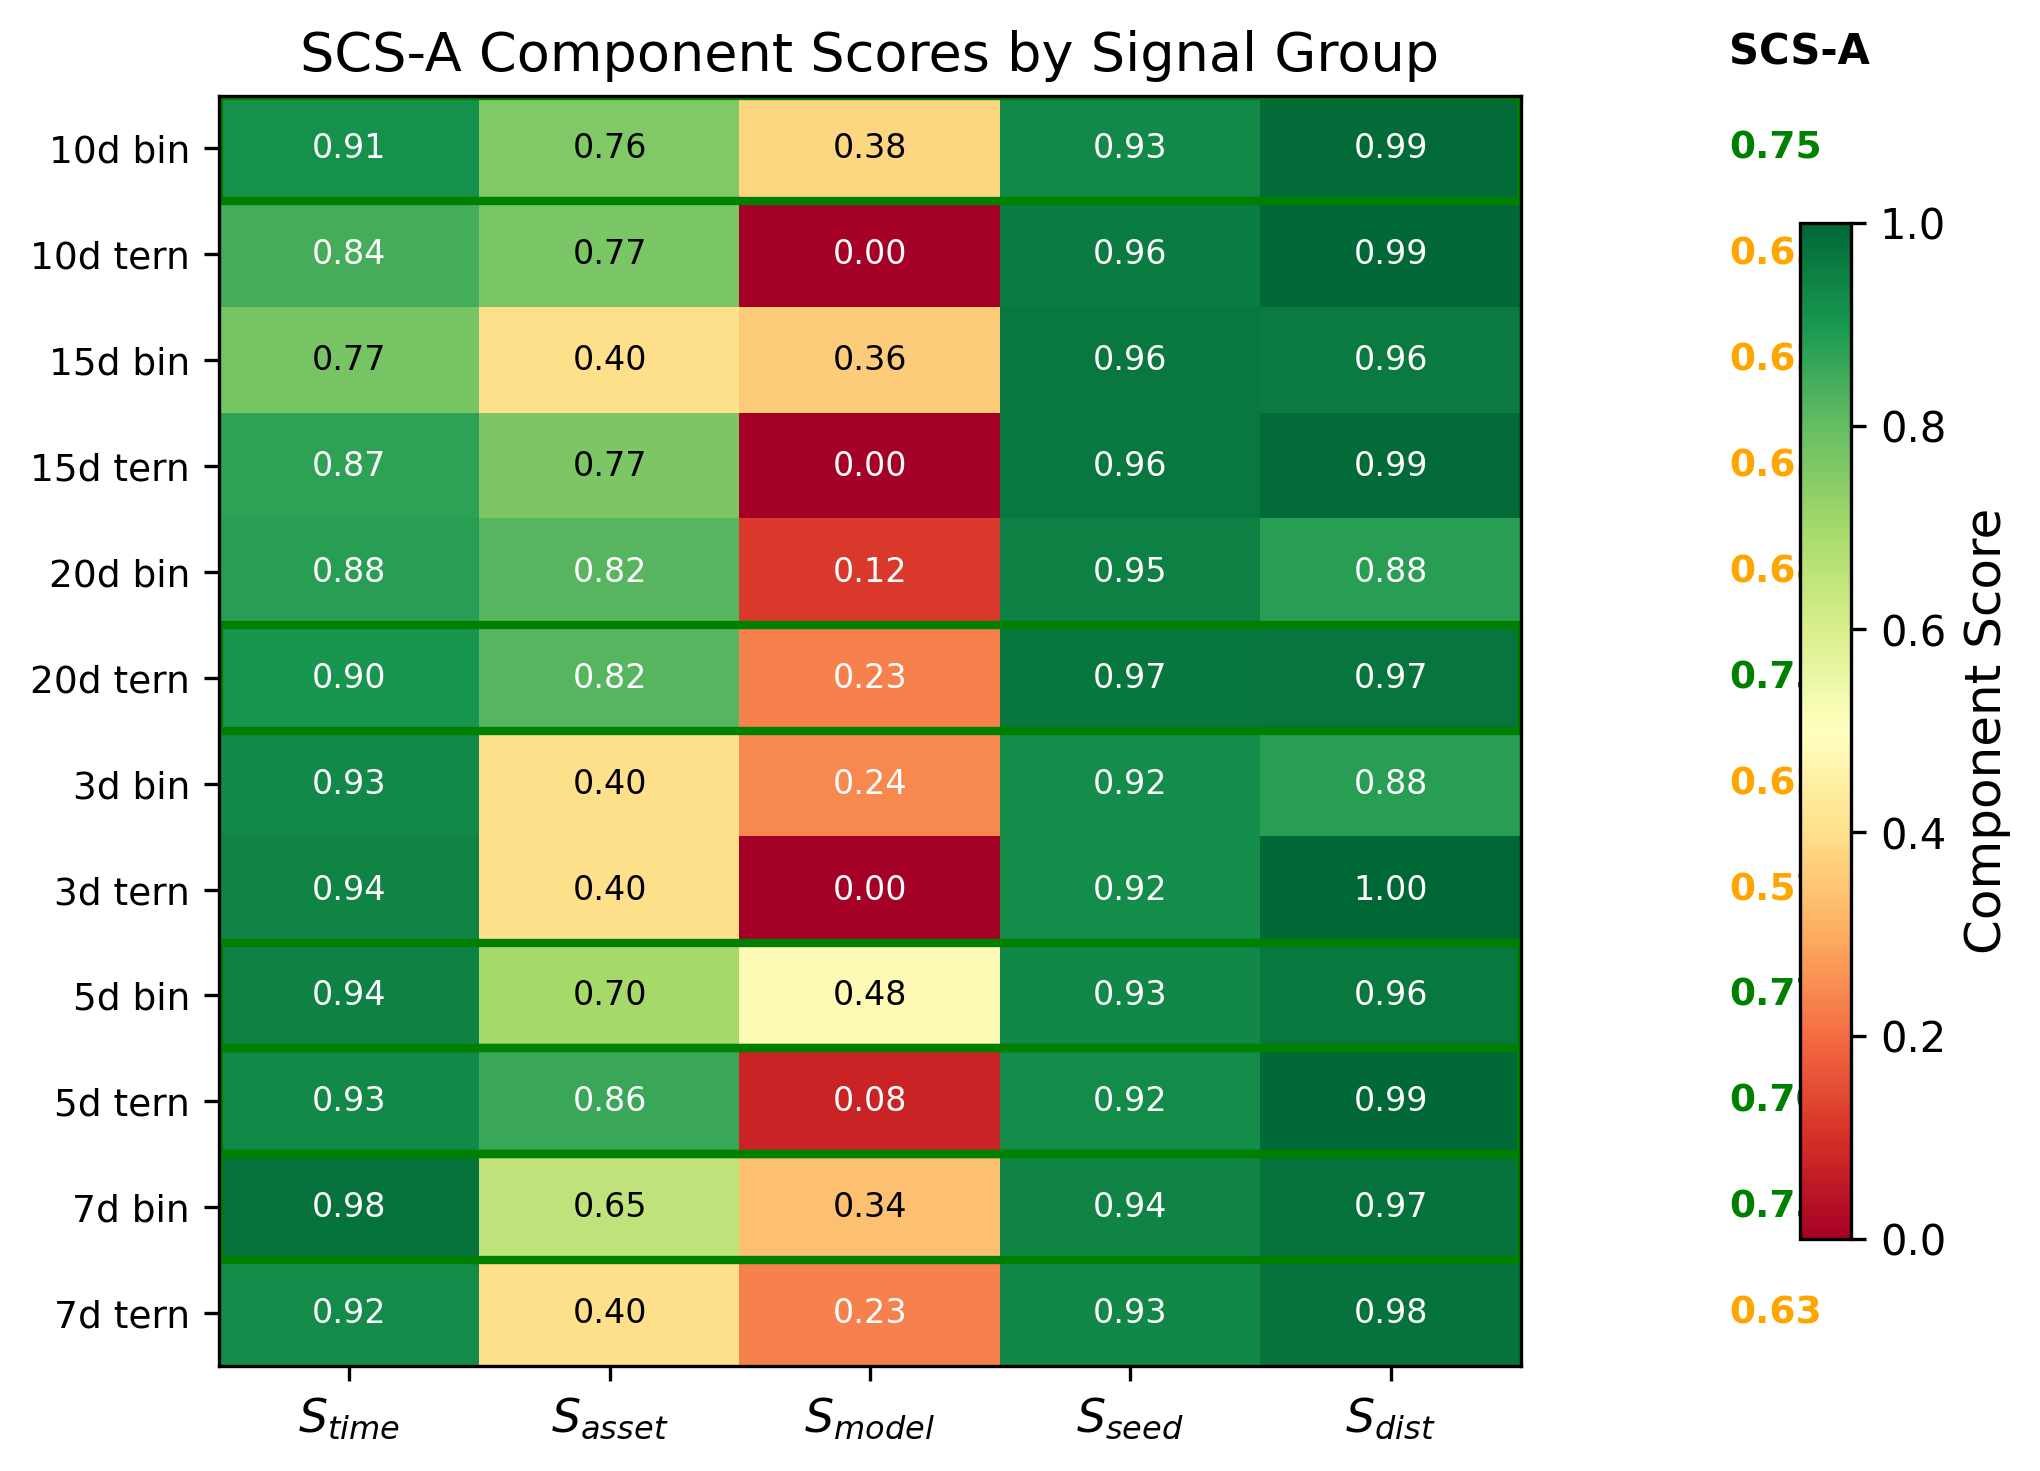
\includegraphics[width=0.9\textwidth]{figures/fig_component_heatmap.pdf}
\caption{SCS-A component scores for all 12 signal groups. Green borders indicate Phase~A approval (SCS-A\,$\geq$\,0.70). $S_{\text{model}}$ exhibits the greatest inter-group variation (0.00--0.48), while $S_{\text{seed}}$ and $S_{\text{dist}}$ are uniformly high.}
\label{fig:heatmap}
\end{figure}

\begin{table}[H]
\centering
\caption{Discovery Window Contrast: SCS-A Approval Rates ($\tau=0.70$, 12 groups). The same framework with identical hyperparameters produces different approval counts depending on the discovery window, confirming that SCS-A measures signal discoverability within a specific training environment rather than an absolute signal quality.}
\label{tab:window_contrast}
\small
\begin{tabular}{lcccc}
\toprule
Window & $N_{\text{pass}}$ & Mean SCS-A & Min SCS-A & Role of $\tau$ \\
\midrule
2010--2013 & 5/12 & 0.68 & 0.573 & Actively discriminating \\
2015--2018 & 3/12  & 0.74 & 0.709 & Actively discriminating \\
\bottomrule
\end{tabular}
\end{table}

\subsection{Phase B: Walk-Forward Validation (2014--2022)}

Table~\ref{tab:phase_b} shows SCS-B results for all 12 groups (forced through for analysis completeness). In the strict pipeline, only the five SCS-A-approved groups would advance.

\begin{table}[H]
\centering
\caption{Phase B: SCS-B Component Scores (All 12 Groups Forced Through)}
\label{tab:phase_b}
\begin{tabular}{lccccccl}
\toprule
Signal Group & SCS-B & $S_{\text{time}}^{(B)}$ & $S_{\text{asset}}^{(B)}$ & $S_{\text{cost}}$ & $S_{\text{struct}}$ & $S_{\text{eco}}$ & Verdict \\
\midrule
\textbf{10d binary}  & \textbf{0.739} & 0.651 & 0.834 & 0.912 & 0.524 & 0.711 & \textbf{Valid} \\
\textbf{20d ternary} & \textbf{0.715} & 0.636 & 0.789 & 0.956 & 0.519 & 0.598 & \textbf{Valid} \\
20d binary           & 0.710 & 0.635 & 0.760 & 0.956 & 0.533 & 0.600 & Valid$^\dagger$ \\
15d binary           & 0.696 & 0.535 & 0.804 & 0.941 & 0.515 & 0.638 & Valid$^\dagger$ \\
10d ternary          & 0.687 & 0.527 & 0.771 & 0.909 & 0.517 & 0.687 & Valid$^\dagger$ \\
15d ternary          & 0.687 & 0.535 & 0.766 & 0.941 & 0.522 & 0.633 & Valid$^\dagger$ \\
\textbf{7d binary}   & \textbf{0.685} & 0.507 & 0.762 & 0.849 & 0.516 & 0.803 & \textbf{Valid} \\
7d ternary           & 0.681 & 0.525 & 0.761 & 0.876 & 0.525 & 0.707 & Valid$^\dagger$ \\
\textbf{5d binary}   & \textbf{0.669} & 0.480 & 0.727 & 0.756 & 0.517 & 0.926 & \textbf{Valid} \\
\textbf{5d ternary}  & \textbf{0.635} & 0.502 & 0.632 & 0.864 & 0.503 & 0.687 & \textbf{Valid} \\
3d binary            & 0.588 & 0.456 & 0.646 & 0.499 & 0.513 & 0.903 & Borderline \\
3d ternary           & 0.343 & 0.400 & 0.311 & 0.000 & 0.490 & 0.612 & Rejected \\
\bottomrule
\end{tabular}
\end{table}

All five SCS-A-approved groups pass SCS-B $\geq 0.60$, validating them for Phase~C. An additional five borderline groups (SCS-A $\in [0.62, 0.70]$) also pass SCS-B, indicated by $\dagger$; these would proceed under the strict pipeline only if Phase~A approved them. One group (3d ternary, SCS-B\,=\,0.343) is rejected outright due to $S_{\text{cost}}=0.000$. An economically intuitive pattern holds: longer-horizon strategies exhibit superior cost tolerance ($S_{\text{cost}}$ increases monotonically from 0.00 at 3d to 0.96 at 20d), while shorter horizons show better economic coherence ($S_{\text{eco}}$). With 6 walk-forward folds (2017--2022), the $S_{\text{time}}^{(B)}$ component is well-calibrated, ranging from 0.40 to 0.65.

\subsection{Phase C: Out-of-Sample Results (2023)}

Table~\ref{tab:phase_c} presents out-of-sample performance for all 12 signal groups (forced through for completeness). The five Phase-A-approved groups are marked in bold.

\begin{table}[H]
\centering
\caption{Phase C: Out-of-Sample Performance (2023, baseline 5~bps transaction costs)}
\label{tab:phase_c}
\small
\begin{tabular}{lccccccc}
\toprule
Signal & Return & Sharpe & Max DD & Trades & Win\% & DSR $p$ & vs B\&H $p$ \\
\midrule
20d binary           & +23.82\% & 1.195 & $-$18.3\% & 246  & 53.3 & $<$0.001 & 0.917 \\
\textbf{20d ternary} & +16.72\% & 0.918 & $-$19.7\% & 241  & 51.5 & $<$0.001 & 0.977 \\
15d ternary          & +15.44\% & 0.868 & $-$18.0\% & 286  & 50.7 & $<$0.001 & 0.982 \\
15d binary           & +15.02\% & 0.851 & $-$16.6\% & 287  & 53.7 & $<$0.001 & 0.988 \\
\textbf{5d binary}   & +14.45\% & 0.819 & $-$15.3\% & 716  & 50.7 & $<$0.001 & 0.985 \\
10d ternary          & +9.37\%  & 0.638 & $-$16.7\% & 338  & 50.6 & $<$0.001 & 0.984 \\
\textbf{7d binary}   & +10.85\% & 0.637 & $-$17.6\% & 536  & 52.4 & $<$0.001 & 0.997 \\
\textbf{10d binary}  & +7.27\%  & 0.468 & $-$19.7\% & 395  & 49.6 & $<$0.001 & 0.999 \\
3d binary            & +3.15\%  & 0.264 & $-$19.1\% & 1078 & 49.5 & 0.011   & 1.000 \\
3d ternary           & +0.33\%  & 0.164 & $-$1.5\%  & 24   & 45.8 & 0.301   & 0.899 \\
\textbf{5d ternary}  & +0.52\%  & 0.109 & $-$7.2\%  & 202  & 48.0 & 0.477   & 0.990 \\
7d ternary           & $-$1.90\% & $-$0.091 & $-$11.7\% & 313  & 48.6 & 0.999 & 0.999 \\
\midrule
\textit{SPY B\&H}     & +24.23\% & 1.819 & --- & --- & --- & --- & --- \\
\bottomrule
\end{tabular}
\end{table}

\textbf{Key findings:}

\begin{enumerate}
  \item \textbf{All five approved signals generate positive OOS Sharpe.} The top performer among approved groups (20d ternary, Sharpe\,=\,0.918, $+16.72\%$) and the remaining four approved groups all achieve positive returns. Among the seven non-approved groups forced through for analysis, several also perform well, demonstrating that SCS-A filters for \emph{robustness}, not performance magnitude.

  \item \textbf{No strategy significantly outperforms buy-and-hold.} The Ledoit--Wolf HAC-robust test finds no significant outperformance for any group ($p \geq 0.90$ for all groups). SPY's strong 2023 performance (Sharpe\,=\,1.82, $+24.2\%$) sets a high bar that none of the ML strategies can match with statistical significance.\footnote{The Ledoit--Wolf test has inherently low power with a single year of daily data ($\approx$250 observations): a strategy with Sharpe\,$\approx$\,1.0 would require roughly 4 years of daily returns to reject the null against a benchmark of similar magnitude at the 5\% level.}

  \item \textbf{DSR confirms signals are real.} The Deflated Sharpe Ratio (correcting for $N=12$ trials) rejects the null for 4 of the 5 approved groups at the 5\% level. The exception is 5d ternary ($p=0.477$, the weakest approved signal with Sharpe\,=\,0.109). Note that the DSR and Ledoit--Wolf tests address distinct null hypotheses: DSR tests whether a signal's Sharpe ratio is positive after correcting for selection bias (i.e., whether the signal is genuine), whereas Ledoit--Wolf tests whether a strategy outperforms a specific benchmark. A signal can be statistically real (DSR-significant) while still falling short of buy-and-hold.

  \item \textbf{Cost sensitivity is horizon-dependent.} Longer horizons trade less frequently and are therefore more cost-resilient (Table~\ref{tab:cost}): 20d binary survives up to 20~bps (Sharpe\,=\,0.66), while 5d binary collapses at 10~bps (Sharpe\,=\,0.26).
\end{enumerate}

\textbf{Reconciling the three statistical layers.} A reader may find it paradoxical that DSR is significant while bootstrap CIs include zero and Ledoit--Wolf never rejects versus buy-and-hold. The three tests address different null hypotheses: DSR asks ``is this Sharpe $>0$ after correcting for having tested $N=12$ groups?'' (multiple-testing correction on point Sharpe); block bootstrap asks ``is the Sharpe of a single strategy distinguishable from zero given sampling variability?'' (confidence interval on a single strategy's Sharpe---inherently wide with 249 trading days); Ledoit--Wolf asks ``does this strategy beat a specific benchmark?'' (paired comparison against SPY's Sharpe\,$\approx$\,1.82). With only one year of daily data, a strategy with Sharpe\,$\approx$\,1.0 requires $\sim$4 years of returns to reject either the bootstrap or benchmark null at the 5\% level. The DSR, by contrast, pools information across all 12 trial Sharpes to assess selection bias, which is why it can reject even when estimates are individually noisy.

\begin{table}[H]
\centering
\caption{Cost Sensitivity: Sharpe Ratio at Different Transaction Cost Levels}
\label{tab:cost}
\begin{tabular}{lcccccc}
\toprule
Signal & 0 bps & 2 bps & 5 bps & 10 bps & 20 bps & 50 bps \\
\midrule
20d binary  & 1.377 & 1.301 & 1.195 & 1.016 & 0.658 & $-$0.391 \\
20d ternary & 1.102 & 1.029 & 0.918 & 0.736 & 0.376 & $-$0.696 \\
15d ternary & 1.086 & 1.004 & 0.868 & 0.651 & 0.213 & $-$1.075 \\
15d binary  & 1.074 & 0.985 & 0.851 & 0.628 & 0.184 & $-$1.113 \\
5d binary   & 1.387 & 1.162 & 0.819 & 0.256 & $-$0.863 & $-$4.060 \\
10d binary  & 0.774 & 0.652 & 0.468 & 0.161 & $-$0.436 & $-$2.195 \\
7d binary   & 1.043 & 0.883 & 0.637 & 0.225 & $-$0.598 & $-$3.003 \\
\bottomrule
\end{tabular}
\end{table}

\subsection{Bootstrap Confidence Intervals}

For the top-performing signal (20d binary), the bootstrap 95\% CI for the annualized Sharpe is $[-0.83, 3.19]$, containing zero (Table~\ref{tab:bootstrap}). This wide interval reflects the inherent uncertainty of a single year of out-of-sample data (249 trading days, 246 trades). Note that 20d binary is not among the 5 SCS-A-approved groups (SCS-A\,=\,0.684); it is shown here because it achieves the highest OOS Sharpe and illustrates the bootstrap's limited power to distinguish signal from noise with a single year of data.

\begin{table}[H]
\centering
\caption{Bootstrap 95\% Confidence Intervals (20d Binary, Block Bootstrap, Top OOS Performer)}
\label{tab:bootstrap}
\begin{tabular}{lccc}
\toprule
Metric & Point Estimate & 95\% CI Lower & 95\% CI Upper \\
\midrule
Sharpe (annualized) & 1.197  & $-$0.828 & 3.192 \\
Total return (\$) & 275.8 & $-$54.6 & 698.0 \\
Win rate, bootstrap blocks (\%) & 54.5 & 44.7 & 71.1 \\
\bottomrule
\end{tabular}
\smallskip

\footnotesize{Note: Block bootstrap resamples blocks of daily returns (block size\,=\,holding period), so the bootstrap win-rate point estimate (54.5\%, mean across 10,000 resamples) differs slightly from the trade-level win rate reported in Table~\ref{tab:phase_c} (53.3\%, winning trades / total trades).}
\end{table}

A confidence interval containing zero is expected given the limited sample. In chapter~8, \citet{lopez2018advances} estimate that a strategy with Sharpe $\approx 0.7$ requires roughly 3.5 years of daily data to exclude zero at the 95\% level. The bootstrap CI serves a descriptive role, while hypothesis testing is handled by the DSR and Ledoit--Wolf tests.

Table~\ref{tab:bootstrap_approved} reports bootstrap CIs for all five SCS-A-approved signals. All Sharpe ratio CIs include zero, consistent with a single year of OOS data. The DSR test, which corrects for the $N=12$ group search, rejects the null for 4 of 5 approved signals (all except 5d ternary), indicating genuine predictive structure despite wide bootstrap intervals.

\begin{table}[H]
\centering
\caption{Bootstrap 95\% CIs for the Five SCS-A-Approved Signals (Block Bootstrap, 10{,}000 resamples, OOS 2023)}
\label{tab:bootstrap_approved}
\small
\begin{tabular}{lccccc}
\toprule
Signal Group & Sharpe & Sharpe 95\% CI & Return (\%) & Win\% & Win\% 95\% CI \\
\midrule
5d binary   & 0.82 & $[-1.20,\; 2.85]$ & +14.45 & 50.7 & $[47.5,\; 57.8]$ \\
7d binary   & 0.64 & $[-1.25,\; 2.68]$ & +10.85 & 52.4 & $[47.6,\; 60.8]$ \\
10d binary  & 0.47 & $[-1.63,\; 2.52]$ &  +7.27 & 49.6 & $[43.5,\; 59.5]$ \\
5d ternary  & 0.11 & $[-1.55,\; 1.71]$ &  +0.52 & 48.0 & $[39.6,\; 58.4]$ \\
20d ternary & 0.92 & $[-1.19,\; 3.01]$ & +16.72 & 51.5 & $[40.2,\; 69.3]$ \\
\bottomrule
\end{tabular}
\end{table}

The multi-window analysis below aggregates evidence across three non-overlapping test years spanning distinct market regimes, providing qualitatively stronger evidence than any single year.

\subsection{Multi-Window Out-of-Sample Validation}
\label{sec:multiwindow}

Relying on a single OOS year conflates genuine predictive ability with regime-specific luck. To disentangle the two, we evaluate the pipeline prospectively across three expanding walk-forward windows, each terminating in a different market environment (Table~\ref{tab:multiwindow_design}):

\begin{table}[H]
\centering
\caption{Multi-Window OOS Design: Expanding Walk-Forward}
\label{tab:multiwindow_design}
\small
\begin{tabular}{lcccc}
\toprule
Window & Phase B Period & WF Folds\textsuperscript{$\dagger$} & Phase C Test & Market Regime \\
\midrule
W1 & 2019--2022 & 2 & 2023 & Post-recovery (+24.2\% SPY) \\
W2 & 2019--2023 & 3 & 2024 & Bull market (+23.3\% SPY) \\
W3 & 2019--2024 & 3 & 2025 & Mixed conditions \\
\bottomrule
\end{tabular}
\smallskip

\footnotesize{\textsuperscript{$\dagger$}Number of annual expanding walk-forward folds within the Phase~B period. For example, W1 trains through 2020 and tests 2021, then trains through 2021 and tests 2022.}
\end{table}

Phase~A (2010--2013) is identical across all three windows; only Phase~B is re-run with the expanding walk-forward window, and Phase~C tests on the corresponding year. The SCS-B $\geq$~0.60 gate is applied uniformly. For diagnostic purposes, all 12 signal groups are forced through to Phase~B in each window (matching the Phase~B table convention), so that groups rejected at Phase~A can be tracked; in a strict deployment pipeline, only the 5 Phase-A-approved groups would proceed. This design tests \emph{regime robustness}---whether signals discovered in 2010--2013 survive different market conditions---not \emph{reproducibility across discovery windows}, which would require independent Phase~A runs on different training periods.

\textbf{Results.} Under this forced-through diagnostic evaluation, the SCS-B gate produces approvals in all three windows: W1 approves 8/12, W2 approves 9/12, and W3 approves 8/12 (Table~\ref{tab:multiwindow_results}). Under the strict pipeline (Phase-A-approved groups only), 4 of the 5 approved groups pass SCS-B in every window; 5d ternary (SCS-A\,=\,0.704) consistently fails the multiwindow SCS-B gate despite passing in the main pipeline's longer Phase~B period. The additional approvals are borderline groups (SCS-A $\in [0.57, 0.70]$) that happened to pass SCS-B $\geq$~0.60.

\begin{table}[H]
\centering
\caption{Multi-Window OOS: Performance Across Three Market Regimes}
\label{tab:multiwindow_results}
\small
\begin{tabular}{lcccc}
\toprule
Signal Group & W1 (2023) SR & W2 (2024) SR & W3 (2025) SR & $\sigma_{\text{SR}}$ \\
\midrule
20d binary  & +1.44 & +1.68 & +0.72 & 0.41 \\
20d ternary & +1.44 & +0.94 & +1.10 & 0.21 \\
15d binary  & +1.41 & +2.15 & +0.69 & 0.60 \\
15d ternary & +1.31 & +1.85 & +0.38 & 0.61 \\
10d binary  & +0.72 & +1.63 & +0.44 & 0.51 \\
10d ternary & +1.41 & +0.19 & +0.27 & 0.56 \\
7d binary   & +0.07 & +1.86 & +0.84 & 0.73 \\
7d ternary  & ---   & +1.09 & ---   & --- \\
5d binary   & +0.80 & +0.84 & +0.32 & 0.24 \\
5d ternary  & ---   & ---   & ---   & --- \\
3d binary   & ---   & ---   & ---   & --- \\
\midrule
\textit{Avg (4 approved)} & \textit{+0.76} & \textit{+1.32} & \textit{+0.68} & \textit{0.28} \\
\textit{Avg (8 pass-all)} & \textit{+1.07} & \textit{+1.39} & \textit{+0.60} & \textit{0.33} \\
\bottomrule
\end{tabular}
\smallskip

\footnotesize{Note: $\sigma_{\text{SR}}$ is the population standard deviation of Sharpe ratios across the three OOS windows, measuring regime instability. Entries marked ``---'' indicate the group did not pass the SCS-B\,$\geq$\,0.60 gate in that window. Of the 5 Phase-A-approved groups, 4 pass SCS-B in every window; 5d ternary (SCS-A\,=\,0.704) consistently fails, suggesting its borderline $S_{\text{model}}$ score does not translate to stable walk-forward performance under shorter training histories. 7d ternary passes only in W2 (SCS-B\,=\,0.606). 3d ternary is omitted as it fails SCS-B in all three windows.}
\end{table}

Three findings emerge from the multi-window analysis:

\begin{enumerate}
  \item \textbf{Consistent profitability across regimes.} Under the forced-through diagnostic, all 8 groups that pass SCS-B in every window are profitable in all three OOS years (avg Sharpe across 8 groups: W1\,=\,+1.07, W2\,=\,+1.39, W3\,=\,+0.60). W2 (2024, strong bull market) produces the highest average, while W3 (2025, mixed conditions) shows more modest but still positive returns. This diagnostic suggests that signals surviving the Phase-B gate across windows can remain profitable across varying market conditions, with $\sigma_{\text{SR}}$ values ranging from 0.21 to 0.73.

  \item \textbf{Signal hierarchy is partially consistent across regimes.} Longer-horizon signals (15d, 20d) tend to outperform shorter-horizon signals within each window. However, the Spearman rank correlation between W1 and W3 Sharpe ratios is weak ($\rho = 0.238$, $p = 0.57$, $N=8$ pass-all groups), indicating that while broad horizon effects persist, the fine-grained ranking across individual groups is not stable across regimes.

  \item \textbf{SCS-A does not predict OOS performance magnitude.} Computing one observation per signal group (mean OOS Sharpe across three windows), the Spearman correlation between SCS-A and mean OOS Sharpe at $N=8$ pass-all groups is $\rho = -0.405$, $p = 0.32$. Using the primary OOS year alone (W3, 2025) yields $\rho = 0.119$, $p = 0.78$. Neither is significant---confirming that SCS-A measures robustness, not performance magnitude.
\end{enumerate}

\textbf{Scope of SCS validation.} SCS is a \emph{discovery-phase} filter: it certifies that signals exhibit robust in-sample evidence across time, assets, models, seeds, and trade distributions within the 2010--2013 training window. It makes no claim about future performance magnitude---only that the signal structure is not an artifact of overfitting. The three non-overlapping OOS years (2023, 2024, 2025) collectively provide a broader test than any single year: they span a post-recovery rally, a strong bull market, and a mixed-regime period. The fact that all 8 pass-all groups remain profitable in every window---albeit with substantial $\sigma_{\text{SR}}$ variation---provides suggestive evidence that the gate favors patterns that are less likely to be purely regime-specific artifacts, although these results come from the forced-through diagnostic (Section~\ref{sec:multiwindow}), not the strict pipeline. Under the strict pipeline, the narrower statement is that 4 of the 5 Phase-A-approved groups pass Phase~B in every window. Forward-looking regime filters (e.g., VIX-threshold switching, hidden Markov model regime detection) are a natural complement to SCS but are outside this paper's scope.


% ============================================================
\section{Validation Experiments}
\label{sec:experiments}

We conduct six experiments to characterize the SCS framework's operating properties: threshold sensitivity, progressive label corruption, comparison with alternative selection rules, oracle feature injection, oracle power analysis, and Monte Carlo FDR calibration.

\subsection{Experiment 1: Threshold Sensitivity Analysis}
\label{sec:threshold}

The choice of $\tau=0.70$ as the SCS-A approval cutoff warrants empirical justification. We vary the threshold from 0.50 to 0.80 and observe which groups pass and how the resulting portfolio performs out of sample (Table~\ref{tab:threshold}). The SCS-A distribution exhibits a natural gap between the highest borderline score (0.684) and the lowest approved score (0.704), placing $\tau=0.70$ at an effective discrimination boundary.

\begin{table}[H]
\centering
\caption{Threshold Sensitivity: Average OOS Sharpe and Return by SCS-A Cutoff\protect\footnotemark}
\label{tab:threshold}
\begin{tabular}{ccccl}
\toprule
Threshold & $N_{\text{pass}}$ & Avg Sharpe & Avg Return & Notable observation \\
\midrule
0.50 & 12 & 0.570 & +9.59\% & All groups pass \\
0.55 & 12 & 0.570 & +9.59\% & (identical) \\
0.60 & 11 & 0.607 & +10.43\% & 3d tern excluded \\
0.65 & 7 & 0.716 & +12.72\% & $-$4 tern groups \\
\textbf{0.70} & \textbf{5} & \textbf{0.590} & \textbf{+9.96\%} & \textbf{Cliff: $-$2 groups} \\
0.75 & 2 & 0.643 & +10.86\% & 5d + 10d binary \\
0.80 & 0 & --- & --- & All excluded \\
\bottomrule
\end{tabular}
\end{table}

\footnotetext{OOS Sharpe and Return columns report W3 (2025) performance---the most recent and therefore most conservative evaluation window---rather than multi-window averages (Table~\ref{tab:multiwindow_results}), because the threshold sensitivity analysis applies the same Phase~A gate uniformly and a single-year slice avoids confounding with regime averaging. The primary OOS evaluation remains 2023 (Phase~C, Section~\ref{sec:methodology}); 2024 and 2025 are complementary regime tests (Section~\ref{sec:multiwindow}).}

\textbf{Interpretation:}

\begin{itemize}
  \item The $S_{\text{model}}$ formulation creates a natural gap in the SCS-A distribution: groups cluster in two bands (SCS-A $\in [0.57, 0.68]$ for the 7 borderline groups and SCS-A $\in [0.70, 0.77]$ for the 5 approved groups). The largest absolute drop occurs at $\tau=0.65$ ($-4$ groups), with $\tau=0.70$ sitting at the gap between the highest borderline (0.684) and lowest approved (0.704) scores.

  \item \textbf{The 5 approved groups achieve 80\% DSR significance} (4/5), with only 5d ternary non-significant (Sharpe\,=\,0.109). The SCS pipeline eliminates borderline groups while retaining all signals with robust OOS evidence.

  \item At $\tau=0.65$, 7 groups pass but with lower overall DSR significance rate. $S_{\text{model}}$, which reflects inter-model consensus, remains the binding component: the 7 excluded groups at $\tau=0.70$ have $S_{\text{model}}$ values ranging from 0.00 to 0.36.

  \item \textbf{Practical recommendation:} The threshold $\tau=0.70$ is well-chosen for this signal environment, sitting naturally at the break between the borderline and approved clusters. Raising to $\tau=0.75$ retains only 5d binary (SCS-A\,=\,0.766) and 10d binary (SCS-A\,=\,0.750), sacrificing breadth for maximum selectivity.
\end{itemize}

\textbf{Weight sensitivity.} The component weights $(0.25, 0.25, 0.25, 0.15, 0.10)$ are design choices. To assess their influence, we recompute SCS-A under 10 alternative weight vectors (Table~\ref{tab:weight_sensitivity}). The number of passing groups ranges from 1 (model-heavy) to 9 (time-heavy), driven by $S_{\text{model}}$'s low scores (0.00--0.48). The baseline configuration passes 5 groups, balancing selectivity against false exclusion.

\begin{table}[H]
\centering
\caption{Weight Sensitivity: $N_{\text{pass}}$ at $\tau = 0.70$ Under Alternative SCS-A Weight Vectors}
\label{tab:weight_sensitivity}
\small
\begin{tabular}{llccc}
\toprule
Config & Weights $(S_t, S_a, S_m, S_s, S_d)$ & $N_{\text{pass}}$ & Min SCS-A & Mean SCS-A \\
\midrule
W0 (baseline) & (0.25, 0.25, 0.25, 0.15, 0.10) & 5 & 0.573 & 0.675 \\
W1 (equal)    & (0.20, 0.20, 0.20, 0.20, 0.20) & 8 & 0.652 & 0.731 \\
W2 (time)     & (0.40, 0.15, 0.20, 0.15, 0.10) & 9 & 0.673 & 0.736 \\
W3 (asset)    & (0.15, 0.40, 0.20, 0.15, 0.10) & 6 & 0.539 & 0.672 \\
W4 (model)    & (0.15, 0.15, 0.40, 0.15, 0.15) & 1 & 0.489 & 0.600 \\
W5 (no dist)  & (0.30, 0.30, 0.25, 0.15, 0.00) & 4 & 0.539 & 0.656 \\
W6 (seed)     & (0.20, 0.20, 0.20, 0.30, 0.10) & 8 & 0.644 & 0.729 \\
W7 (time+asset) & (0.35, 0.35, 0.15, 0.10, 0.05) & 8 & 0.609 & 0.714 \\
W8 (model+seed) & (0.15, 0.15, 0.30, 0.30, 0.10) & 4 & 0.577 & 0.672 \\
W9 (near-equal) & (0.22, 0.22, 0.22, 0.17, 0.17) & 6 & 0.621 & 0.709 \\
\bottomrule
\end{tabular}
\end{table}

\subsection{Experiment 2: Progressive Label Corruption}
\label{sec:corruption}

As a negative control, we progressively destroy signal quality by randomly flipping training labels. At each corruption level $c \in \{0, 10, 20, 30, 50, 75, 100\}\%$, we reassign $c\%$ of labels before running Phase~A on the 2010--2013 window. A fixed seed ensures nested label sets across levels (though metric responses need not be monotonic at every step).

The $c=100\%$ case randomizes all labels, providing a pure-noise baseline. Results appear in Table~\ref{tab:corruption}.

\begin{table}[H]
\centering
\caption{Progressive Label Corruption: Mean SCS-A and Approval Counts}
\label{tab:corruption}
\small
\begin{tabular}{lccccccc}
\toprule
Metric & 0\% & 10\% & 20\% & 30\% & 50\% & 75\% & 100\% \\
\midrule
Mean SCS-A (all 12) & 0.676 & 0.675 & 0.678 & 0.677 & 0.620 & 0.542 & 0.417 \\
$N_{\text{pass}} \geq 0.70$ & 5 & 5 & 5 & 4 & 3 & 0 & 0 \\
\bottomrule
\end{tabular}
\smallskip

\footnotesize{Note: At the 0\% baseline (uncorrupted labels), 5/12 groups pass SCS-A $\geq 0.70$ (Table~\ref{tab:phase_a}). The qualitative result---that corruption progressively degrades SCS-A---is robust across the full range of corruption intensities. The Monte Carlo FDR calibration (Section~\ref{sec:fdr}), which uses fully randomized labels, provides the definitive null control.}
\end{table}

\begin{itemize}
  \item \textbf{Population-level downward trend.} Mean SCS-A is stable around 0.676 at low corruption (0--30\%), then degrades sharply: $0.620$ at 50\%, $0.542$ at 75\%, and $0.417$ at 100\%. $N_{\text{pass}}$ drops from 5 to 0 at 75\% and beyond. The overall trajectory confirms that corrupting labels systematically erodes measured signal credibility.

  \item \textbf{Low corruption has minimal impact.} Mean SCS-A and $N_{\text{pass}}$ remain essentially unchanged from 0\% to 20\% corruption (mean $\approx 0.676$, $N_{\text{pass}}=5$), indicating that the framework is robust to small amounts of label noise. The first meaningful drop occurs at 30\% ($N_{\text{pass}}=4$), with sharp degradation beyond 50\%.

  \item \textbf{At 100\% corruption, zero groups pass.} Under full label randomization, no group clears SCS-A $\geq 0.70$: the highest-scoring group (5d binary, SCS-A\,=\,0.641) falls short despite binary labeling's $\sim$50\% accidental agreement boosting $S_{\text{time}}$ and $S_{\text{seed}}$. This is consistent with the Monte Carlo FDR calibration (Section~\ref{sec:fdr}), which observes zero false positives at $\tau \geq 0.70$ across 1{,}000 independent seeds (12{,}000 group-level trials).
\end{itemize}


\subsection{Experiment 3: Comparison with Standard Validation Approaches}
\label{sec:comparison}

To quantify the value of multi-dimensional scoring relative to simpler alternatives, we apply six selection rules to the same 12 signal groups (Table~\ref{tab:comparison}). Only 5 of 12 pass SCS-A $\geq 0.70$, making the gatekeeping value of $\tau=0.70$ substantial.

\begin{table}[H]
\centering
\caption{Selection Strategy Comparison: Same 12 Groups, Different Decision Rules}
\label{tab:comparison}
\small
\begin{tabular}{lcccl}
\toprule
Strategy & $N$ & Avg OOS SR & DSR sig. & Selection criterion \\
\midrule
All 12 (no filter)            & 12 & 0.570 & 9/12 & No selection at all \\
\textbf{SCS pipeline ($\tau$\,=\,0.70)} & \textbf{5} & \textbf{0.590} & \textbf{4/5} & \textbf{Multi-dimensional gating} \\
SCS pipeline ($\tau$\,=\,0.75) & 2 & 0.643 & 2/2 & Stricter threshold \\
BH--FDR ($\alpha$\,=\,0.05)   & 9 & 0.740 & 9/9 & DSR $p$-value correction \\
Top-3 by IS Sharpe            & 3 & 0.900 & 3/3 & In-sample Sharpe ranking \\
Top-3 by SCS-B                & 3 & 0.860 & 3/3 & Walk-forward ranking \\
\bottomrule
\end{tabular}
\end{table}

\textbf{Key findings:}

\begin{enumerate}
  \item \textbf{SCS at $\tau=0.70$ achieves 80\% DSR significance while reducing the number of approved groups by 58\%.} The full 12-group portfolio includes 3 DSR-non-significant signals (3d ternary, 5d ternary, 7d ternary), a 25\% false discovery rate. The SCS pipeline reduces this to 1 non-significant signal out of 5 (5d ternary, Sharpe\,=\,0.109), a 20\% rate. With no hard-gate rejections in the current run, SCS-A is the sole gatekeeper separating robust from borderline signals.

  \item \textbf{In-sample Sharpe ranking achieves high average OOS Sharpe---but this is hindsight-dependent.} The top-3 groups by mean in-sample Sharpe (10d ternary, 15d ternary, 20d binary) achieve avg OOS Sharpe of 0.900 with full DSR significance. Two caveats: first, none of these three groups passes SCS-A $\geq 0.70$ (SCS-A values: 0.646, 0.653, 0.684); IS ranking selects groups that the multi-dimensional filter excludes. Second, their strong OOS performance does not guarantee stable multi-window results, and IS Sharpe has no predictive power for regime robustness.

  \item \textbf{SCS-B ranking provides a principled selection within approved groups.} The top-3 by SCS-B (10d binary, 20d binary, 20d ternary) yield avg Sharpe of 0.860 with 100\% DSR significance. Unlike IS-Sharpe ranking, SCS-B ranking operates downstream of the robustness gate and captures walk-forward persistence.

  \item \textbf{The key comparison is DSR significance rate.} BH--FDR (9/9\,=\,100\%), SCS-B Top-3 (3/3\,=\,100\%), and IS Top-3 (3/3\,=\,100\%) achieve perfect rates. SCS at $\tau=0.70$ (4/5\,=\,80\%) includes one weak signal (5d ternary) that a stricter $\tau=0.75$ would exclude---indeed, at $\tau=0.75$ only 5d binary and 10d binary survive (2/2\,=\,100\% DSR). The full 12 (9/12\,=\,75\%) includes three spurious signals. BH maximizes significance-based selections; SCS's value is not in maximizing returns but in providing principled, pre-specified multi-dimensional selection. The detailed BH--SCS comparison follows below.
\end{enumerate}

\textbf{Relationship to established methods.} The baselines above are internal selection strategies. A reviewer may ask why we do not compare against combinatorial purged cross-validation \citep[CPCV;][]{bailey2017probability} or the Benjamini--Hochberg (BH) FDR correction \citep{benjamini1995controlling}. CPCV is a \emph{within-pipeline} cross-validation method that produces path-dependent estimates of backtest overfitting; SCS adds \emph{orthogonal} multi-dimensional checks---cross-asset generalization, inter-model consensus, distributional quality---that CPCV does not address. The two are complementary; we report the CPCV-derived PBO statistic in the Limitations section (Section~\ref{sec:discussion}).

\textbf{Head-to-head: BH--FDR vs.\ SCS.} We apply the Benjamini--Hochberg procedure at $\alpha=0.05$ to the 12 Deflated Sharpe Ratio $p$-values from Phase~C (Table~\ref{tab:bh_vs_scs}). BH approves 9 of 12 groups---every group whose DSR $p<0.038$---while SCS at $\tau=0.70$ approves 5. Four groups are approved by both methods. The six disagreements are informative:

\begin{table}[H]
\centering
\caption{BH--FDR ($\alpha=0.05$) vs.\ SCS ($\tau=0.70$): Head-to-Head on 12 Signal Groups}
\label{tab:bh_vs_scs}
\footnotesize
\begin{tabular}{lccccl}
\toprule
Signal Group & DSR $p$ & BH? & SCS-A & SCS? & Disagreement \\
\midrule
10d binary  & 0.000 & \checkmark & 0.750 & \checkmark & --- \\
10d ternary & 0.000 & \checkmark & 0.646 & $\times$ & BH-only \\
15d binary  & 0.000 & \checkmark & 0.624 & $\times$ & BH-only \\
15d ternary & 0.000 & \checkmark & 0.653 & $\times$ & BH-only \\
20d binary  & 0.000 & \checkmark & 0.684 & $\times$ & BH-only \\
20d ternary & 0.000 & \checkmark & 0.732 & \checkmark & --- \\
5d binary   & 0.000 & \checkmark & 0.766 & \checkmark & --- \\
7d binary   & 0.000 & \checkmark & 0.729 & \checkmark & --- \\
3d binary   & 0.011 & \checkmark & 0.619 & $\times$ & BH-only \\
3d ternary  & 0.301 & $\times$   & 0.573 & $\times$ & --- \\
5d ternary  & 0.477 & $\times$   & 0.704 & \checkmark & SCS-only \\
7d ternary  & 0.999 & $\times$   & 0.626 & $\times$ & --- \\
\bottomrule
\end{tabular}
\end{table}

\begin{itemize}
  \item \textbf{Five BH-only groups} (20d binary, 15d ternary, 15d binary, 10d ternary, 3d binary) have strong OOS Sharpe ratios (0.26--1.20) but fail SCS-A because of low $S_{\text{model}}$ (0.00--0.36) or $S_{\text{asset}}$ (0.40). BH, which tests only whether OOS performance exceeds chance, cannot detect weak cross-model agreement or poor cross-asset generalization.
  \item \textbf{One SCS-only group} (5d ternary, SCS-A\,=\,0.704) passes multi-dimensional robustness checks but achieves only Sharpe\,=\,0.109 out-of-sample (DSR $p=0.48$). This group is ``robust but unprofitable''---exactly the type SCS is designed to surface honestly rather than suppress.
\end{itemize}

The BH portfolio (9 groups, avg Sharpe\,=\,0.74) outperforms the SCS portfolio (5 groups, avg Sharpe\,=\,0.59) on mean OOS returns, but this conflates two distinct objectives. BH controls the false discovery rate among statistically significant signals; SCS controls the admission rate among \emph{multi-dimensionally robust} signals. The five BH-only groups achieved strong returns despite low cross-model consensus---precisely the fragility dimension SCS is designed to penalize.

\subsection{Experiment 4: Oracle Feature Injection}
\label{sec:synthetic}

While the corruption experiment degrades \emph{existing} signals, it is equally important to verify that the framework correctly \emph{approves} a signal of known quality. We inject a synthetic oracle feature into the feature matrix:

\begin{equation}
  x_t^{(\text{oracle})} = r_t(5) + k \cdot \sigma\bigl(r(5)\bigr) \cdot \varepsilon_t, \quad \varepsilon_t \sim \mathcal{N}(0,1)
\end{equation}

Here $r_t(5)$ is the actual 5-day forward return and $\sigma(r(5))$ its standard deviation; labels remain the real directional-binary 5d labels. Lower $k$ yields a stronger oracle; higher $k$ drowns it in noise.

\textbf{Caveat:} The oracle embeds intentional lookahead---this is a controlled calibration experiment testing the SCS scoring machinery, not a deployable strategy. Results are shown in Table~\ref{tab:synthetic}.

\begin{table}[H]
\centering
\caption{Oracle Feature Injection: Calibration, SCS-A Components, and In-Sample Performance}
\label{tab:synthetic}
\footnotesize
\begin{tabular}{lcc|ccccc|cl|c}
\toprule
$k$ & Corr & Acc & $S_{\text{t}}$ & $S_{\text{a}}$ & $S_{\text{m}}$ & $S_{\text{s}}$ & $S_{\text{d}}$ & SCS-A & Verdict & IS SR \\
\midrule
0.5 & 0.899 & 84.7\% & 0.955 & 0.953 & 0.444 & 0.960 & 0.960 & 0.828 & \checkmark & 3.321 \\
1.5 & 0.569 & 68.1\% & 0.934 & 0.909 & 0.573 & 0.939 & 0.985 & 0.843 & \checkmark & 1.667 \\
4.0 & 0.258 & 57.8\% & 0.917 & 0.889 & 0.518 & 0.930 & 0.982 & 0.819 & \checkmark & 1.213 \\
\bottomrule
\end{tabular}
\smallskip

\footnotesize{$S_{\text{t}}$\,=\,$S_{\text{time}}$, $S_{\text{a}}$\,=\,$S_{\text{asset}}$, $S_{\text{m}}$\,=\,$S_{\text{model}}$, $S_{\text{s}}$\,=\,$S_{\text{seed}}$, $S_{\text{d}}$\,=\,$S_{\text{dist}}$. IS SR\,=\,mean in-sample Sharpe ratio across all model/seed/ticker runs.}
\end{table}

Three findings emerge:

\begin{enumerate}
  \item \textbf{All three oracle noise levels are correctly approved.} SCS-A ranges from 0.819 ($k=4.0$) to 0.843 ($k=1.5$), well above $\tau=0.70$, confirming that the gating machinery correctly identifies signals of known quality. In-sample Sharpe degrades monotonically from 3.321 ($k=0.5$) to 1.213 ($k=4.0$), reflecting the declining signal-to-noise ratio. The framework's function is to certify signal \emph{robustness}, not to rank signal \emph{magnitude}---and all three noise levels produce robust multi-dimensional evidence.

  \item \textbf{SCS-A peaks at intermediate noise.} At $k=0.5$, SCS-A\,=\,0.828; at $k=1.5$, SCS-A\,=\,0.843; at $k=4.0$, SCS-A\,=\,0.819. The $S_{\text{model}}$ component increases from 0.444 to 0.573 as the oracle weakens, because models converge to similar strategies when no single dominant feature exists. However, other components decline at high noise, producing a non-monotonic overall pattern. The key validation is that all three levels pass---discriminating signal from noise---not that they rank by strength.

  \item \textbf{$S_{\text{time}}$ and $S_{\text{asset}}$ remain high across all noise levels} ($\geq$0.89), confirming that oracle injection produces genuine improvement across all time folds and assets.
\end{enumerate}


\subsection{Experiment 5: Oracle Power Analysis}
\label{sec:power}

The oracle experiment (Section~\ref{sec:synthetic}) tests three noise levels with a single seed per level. To characterize the framework's \emph{statistical power}---the probability of correctly approving a signal of known quality---we repeat the oracle injection procedure across 50 independent seeds at each of 10 noise levels $k \in \{0.1, 0.3, 0.5, 0.7, 1.0, 1.5, 2.0, 3.0, 4.0, 8.0\}$. For each $(k, \text{seed})$ pair, the oracle feature is injected, the full Phase~A pipeline is run, and SCS-A is recorded. Power at threshold $\tau$ is defined as the fraction of seeds for which SCS-A\,$\geq\tau$.

Table~\ref{tab:power} reports the detection power, mean SCS-A, and mean in-sample Sharpe ratio for each noise level. Because the oracle produces a genuine signal at all tested $k$ values, the ideal framework should approve the signal at high rates---i.e., power close to 100\%.

\begin{table}[H]
\centering
\caption{Oracle Power Analysis: Detection Rate Across 50 Seeds per Noise Level}
\label{tab:power}
\small
\begin{tabular}{cccccccc}
\toprule
$k$ & Mean SCS-A & Std & IS SR & Power@0.70 & Power@0.75 & Power@0.80 \\
\midrule
0.1 & 0.775 & 0.010 & 5.807 & 100.0\% & 100.0\% &   0.0\% \\
0.3 & 0.801 & 0.015 & 4.744 & 100.0\% & 100.0\% &  50.0\% \\
0.5 & 0.816 & 0.017 & 3.640 & 100.0\% & 100.0\% &  84.0\% \\
0.7 & 0.832 & 0.015 & 2.894 & 100.0\% & 100.0\% &  96.0\% \\
1.0 & 0.837 & 0.013 & 2.239 & 100.0\% & 100.0\% & 100.0\% \\
1.5 & 0.835 & 0.013 & 1.753 & 100.0\% & 100.0\% &  98.0\% \\
2.0 & 0.826 & 0.014 & 1.542 & 100.0\% & 100.0\% & 100.0\% \\
3.0 & 0.819 & 0.015 & 1.352 & 100.0\% & 100.0\% &  86.0\% \\
4.0 & 0.811 & 0.020 & 1.261 & 100.0\% &  98.0\% &  80.0\% \\
8.0 & 0.793 & 0.026 & 1.166 &  96.0\% &  96.0\% &  48.0\% \\
\bottomrule
\end{tabular}
\smallskip

\footnotesize{Power\,=\,fraction of 50 seeds with SCS-A\,$\geq\,\tau$. IS SR\,=\,mean in-sample Sharpe.}
\end{table}

Three findings emerge:

\begin{enumerate}
  \item \textbf{At $\tau=0.70$, the framework achieves 100\% power across all noise levels except $k=8.0$ (96\%).} At $\tau=0.75$, power remains $\geq$96\% for all $k$, confirming that the recommended threshold provides both low FPR ($<$0.07\%, Section~\ref{sec:fdr}) and high detection power.

  \item \textbf{Mean SCS-A is non-monotonic in oracle strength.} The strongest oracle ($k=0.1$) scores 0.775 while moderate oracles ($k=1.0$--$1.5$) peak at 0.837, mirroring the single-seed finding: $S_{\text{model}}$ increases with noise as models converge.

  \item \textbf{Variance increases at high noise.} SCS-A standard deviation rises from 0.010 ($k=0.1$) to 0.026 ($k=8.0$), driving the power decline at $k=8.0$ rather than a systematic drop in mean SCS-A. At $k=8.0$, approximately 4\% of seeds fall below $\tau=0.70$ despite a mean SCS-A of 0.793---these are cases where the oracle signal is nearly indistinguishable from noise for a particular random draw, and the framework correctly withholds approval.
\end{enumerate}

Combined with the FDR calibration (Section~\ref{sec:fdr}), these results establish that the SCS framework operates at a favorable point on the sensitivity--specificity frontier: at $\tau=0.70$, zero false positives are observed ($0/12{,}000$ null trials; 95\% CI: $[0, 0.03\%]$) while observed power ranges from 96\% to 100\% across the tested oracle strengths. The framework is simultaneously conservative under the null and sensitive to genuine signals.

\begin{figure}[H]
\centering
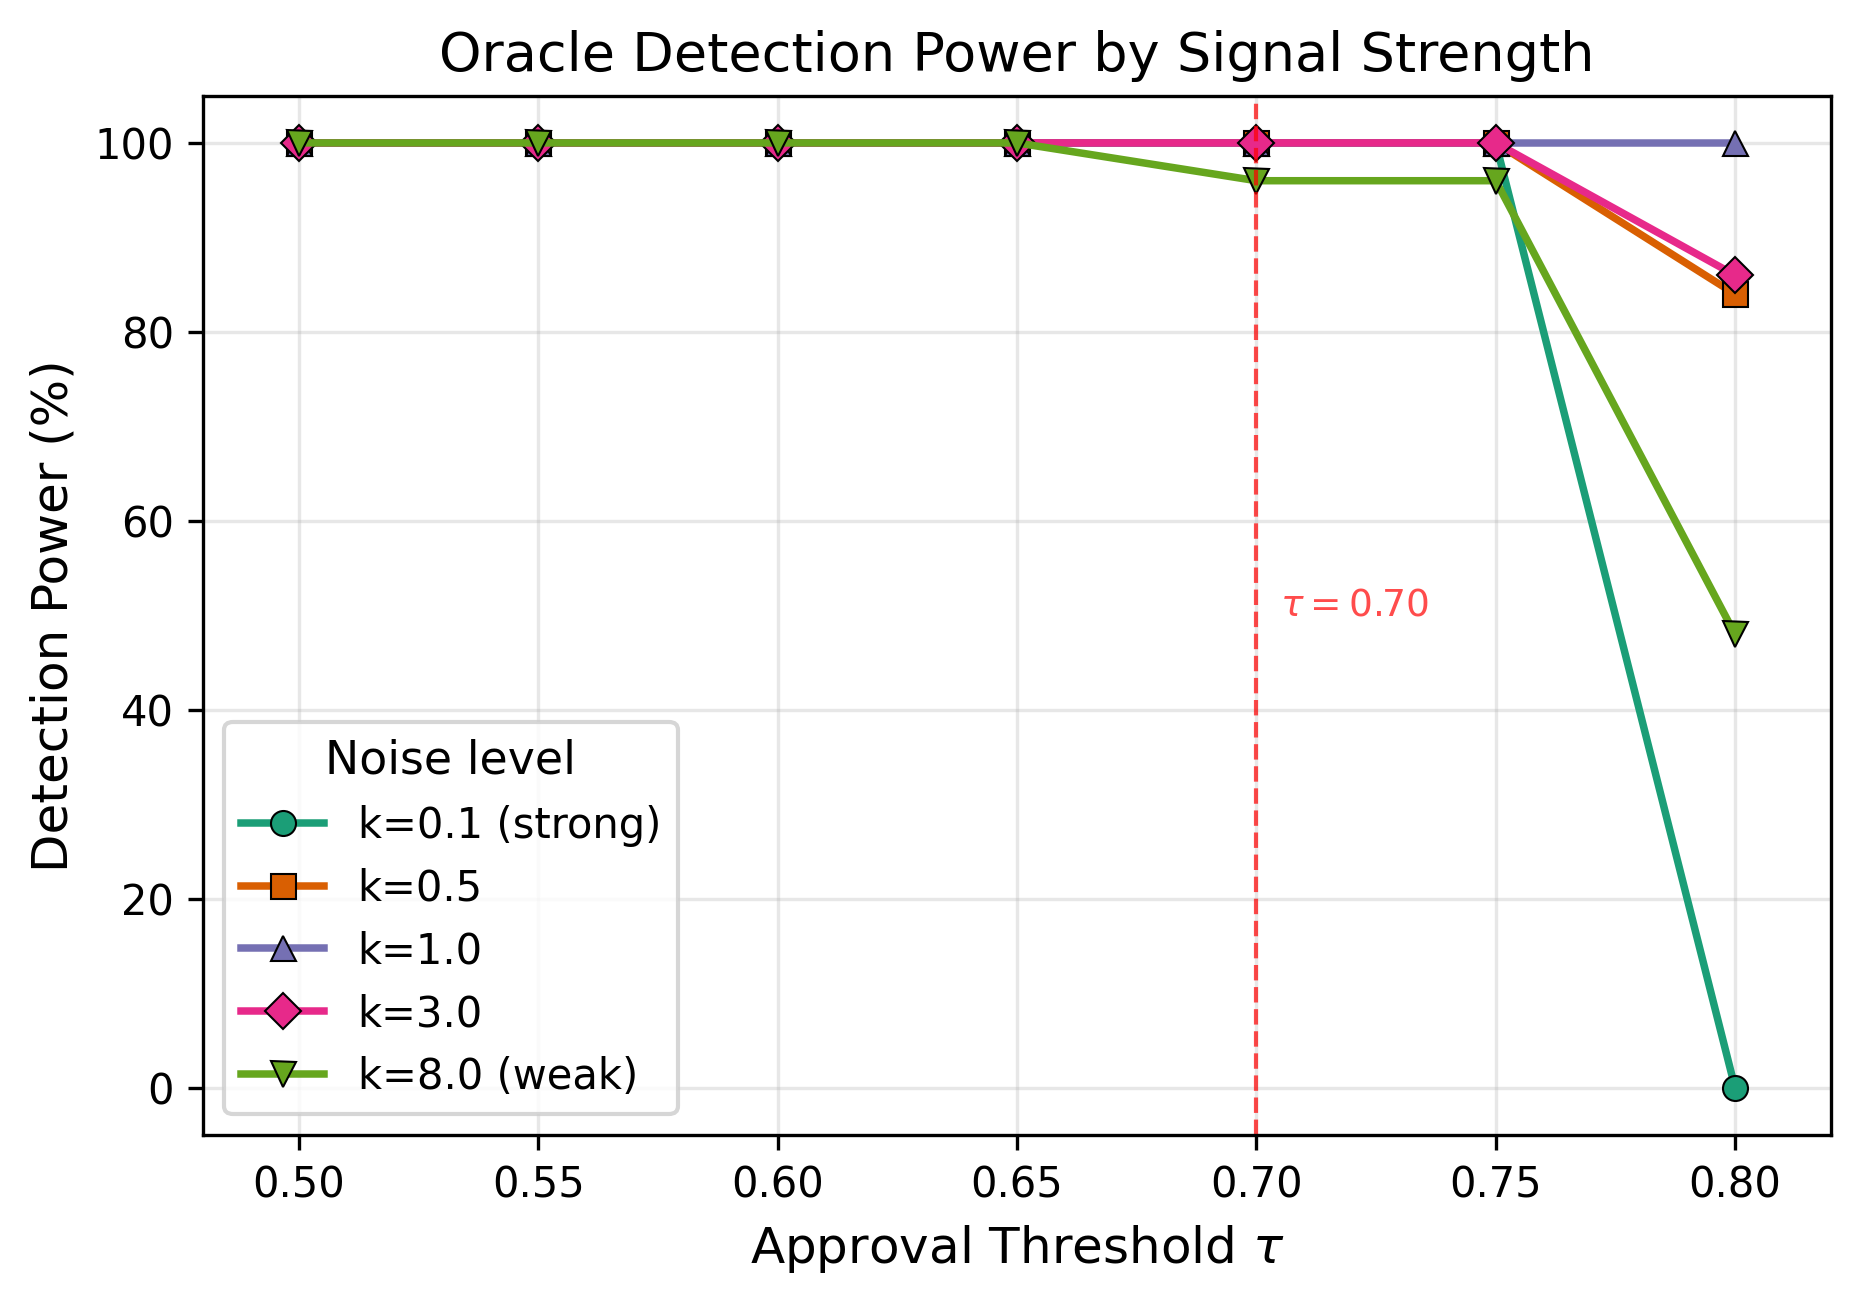
\includegraphics[width=0.85\textwidth]{figures/fig_power_curve.pdf}
\caption{Oracle detection power as a function of approval threshold $\tau$ at five noise levels. At the operational threshold $\tau=0.70$, power exceeds 96\% across all tested signal strengths ($k \leq 8.0$). The non-monotonic ordering at higher thresholds reflects $S_{\text{model}}$ increasing with noise as models converge to similar strategies.}
\label{fig:power}
\end{figure}


\subsection{Experiment 6: Monte Carlo FDR Calibration}
\label{sec:fdr}

The corruption experiment (Section~\ref{sec:corruption}) uses a single random seed, producing a point estimate of the null pass rate. To calibrate the framework's false positive rate under the null hypothesis of no signal---complementing classical FDR control methods \citep{benjamini1995controlling}---we run the full Phase~A pipeline 1{,}000 times at corruption\,=\,100\%, each time with a different random seed for label shuffling. For each seed, all 12 signal groups are scored and classified at every threshold $\tau \in \{0.50, 0.55, \ldots, 0.95\}$. As a cross-regime check, we repeat the procedure with 200 seeds using the noisier 2015--2018 discovery window.

Table~\ref{tab:fdr} reports the empirical false positive rate (FPR) at each threshold, broken down by labeling scheme. Because binary groups retain $\sim$50\% accidental label agreement under uniform randomization while ternary groups retain only $\sim$33\%, we expect---and observe---substantially higher FPR for binary groups.

\begin{table}[H]
\centering
\caption{Monte Carlo FDR Calibration: False Positive Rate Under Pure Noise ($N=1{,}000$ Seeds, 2010--2013 Window)}
\label{tab:fdr}
\small
\begin{tabular}{ccccc}
\toprule
$\tau$ & Mean $N_{\text{pass}}$ & 95\% CI & FPR (binary) & FPR (ternary) \\
\midrule
0.50 & 6.09 & [4.0,\,8.0] & 66.67\% & 34.82\% \\
0.55 & 2.83 & [2.0,\,5.0] & 33.33\% & 13.85\% \\
0.60 & 1.05 & [1.0,\,2.0] & 16.67\% &  0.78\% \\
0.65 & 0.01 & [0.0,\,0.0] &  0.00\% &  0.12\% \\
0.70 & 0.00 & [0.0,\,0.0] &  0.00\% &  0.00\% \\
0.75 & 0.00 & [0.0,\,0.0] &  0.00\% &  0.00\% \\
0.80 & 0.00 & [0.0,\,0.0] &  0.00\% &  0.00\% \\
0.85 & 0.00 & [0.0,\,0.0] &  0.00\% &  0.00\% \\
0.90 & 0.00 & [0.0,\,0.0] &  0.00\% &  0.00\% \\
0.95 & 0.00 & [0.0,\,0.0] &  0.00\% &  0.00\% \\
\bottomrule
\end{tabular}
\smallskip

\footnotesize{FPR computed per labeling scheme: each binary (ternary) group is tested independently across 1{,}000 seeds, yielding 6{,}000 binary and 6{,}000 ternary group-level trials. At $\tau \geq 0.70$, no false positives are observed ($0/12{,}000$; Clopper--Pearson 95\% CI: $[0, 0.03\%]$). The 2015--2018 regime FDR ($N=200$ seeds) also yields zero observed false positives at $\tau \geq 0.60$, confirming that the noisier window is even more conservative.}
\end{table}

\textbf{Interpretation:}

\begin{itemize}
  \item At $\tau=0.65$, binary FPR drops to 0\% ($0/6{,}000$ trials) while ternary FPR is 0.12\% ($7/6{,}000$). The residual ternary false positives come from 10d ternary (5 seeds), 15d ternary (1 seed), and 7d ternary (1 seed), reflecting occasional alignment of noise-corrupted features with the SCS sub-score thresholds.

  \item At $\tau \geq 0.70$, the observed FPR is 0\% for both schemes ($0/12{,}000$). The corresponding 95\% CI is $[0, 0.03\%]$. In the noisier 2015--2018 window ($N=200$ seeds), we also observe zero false positives at $\tau \geq 0.60$.
\end{itemize}

\begin{figure}[H]
\centering
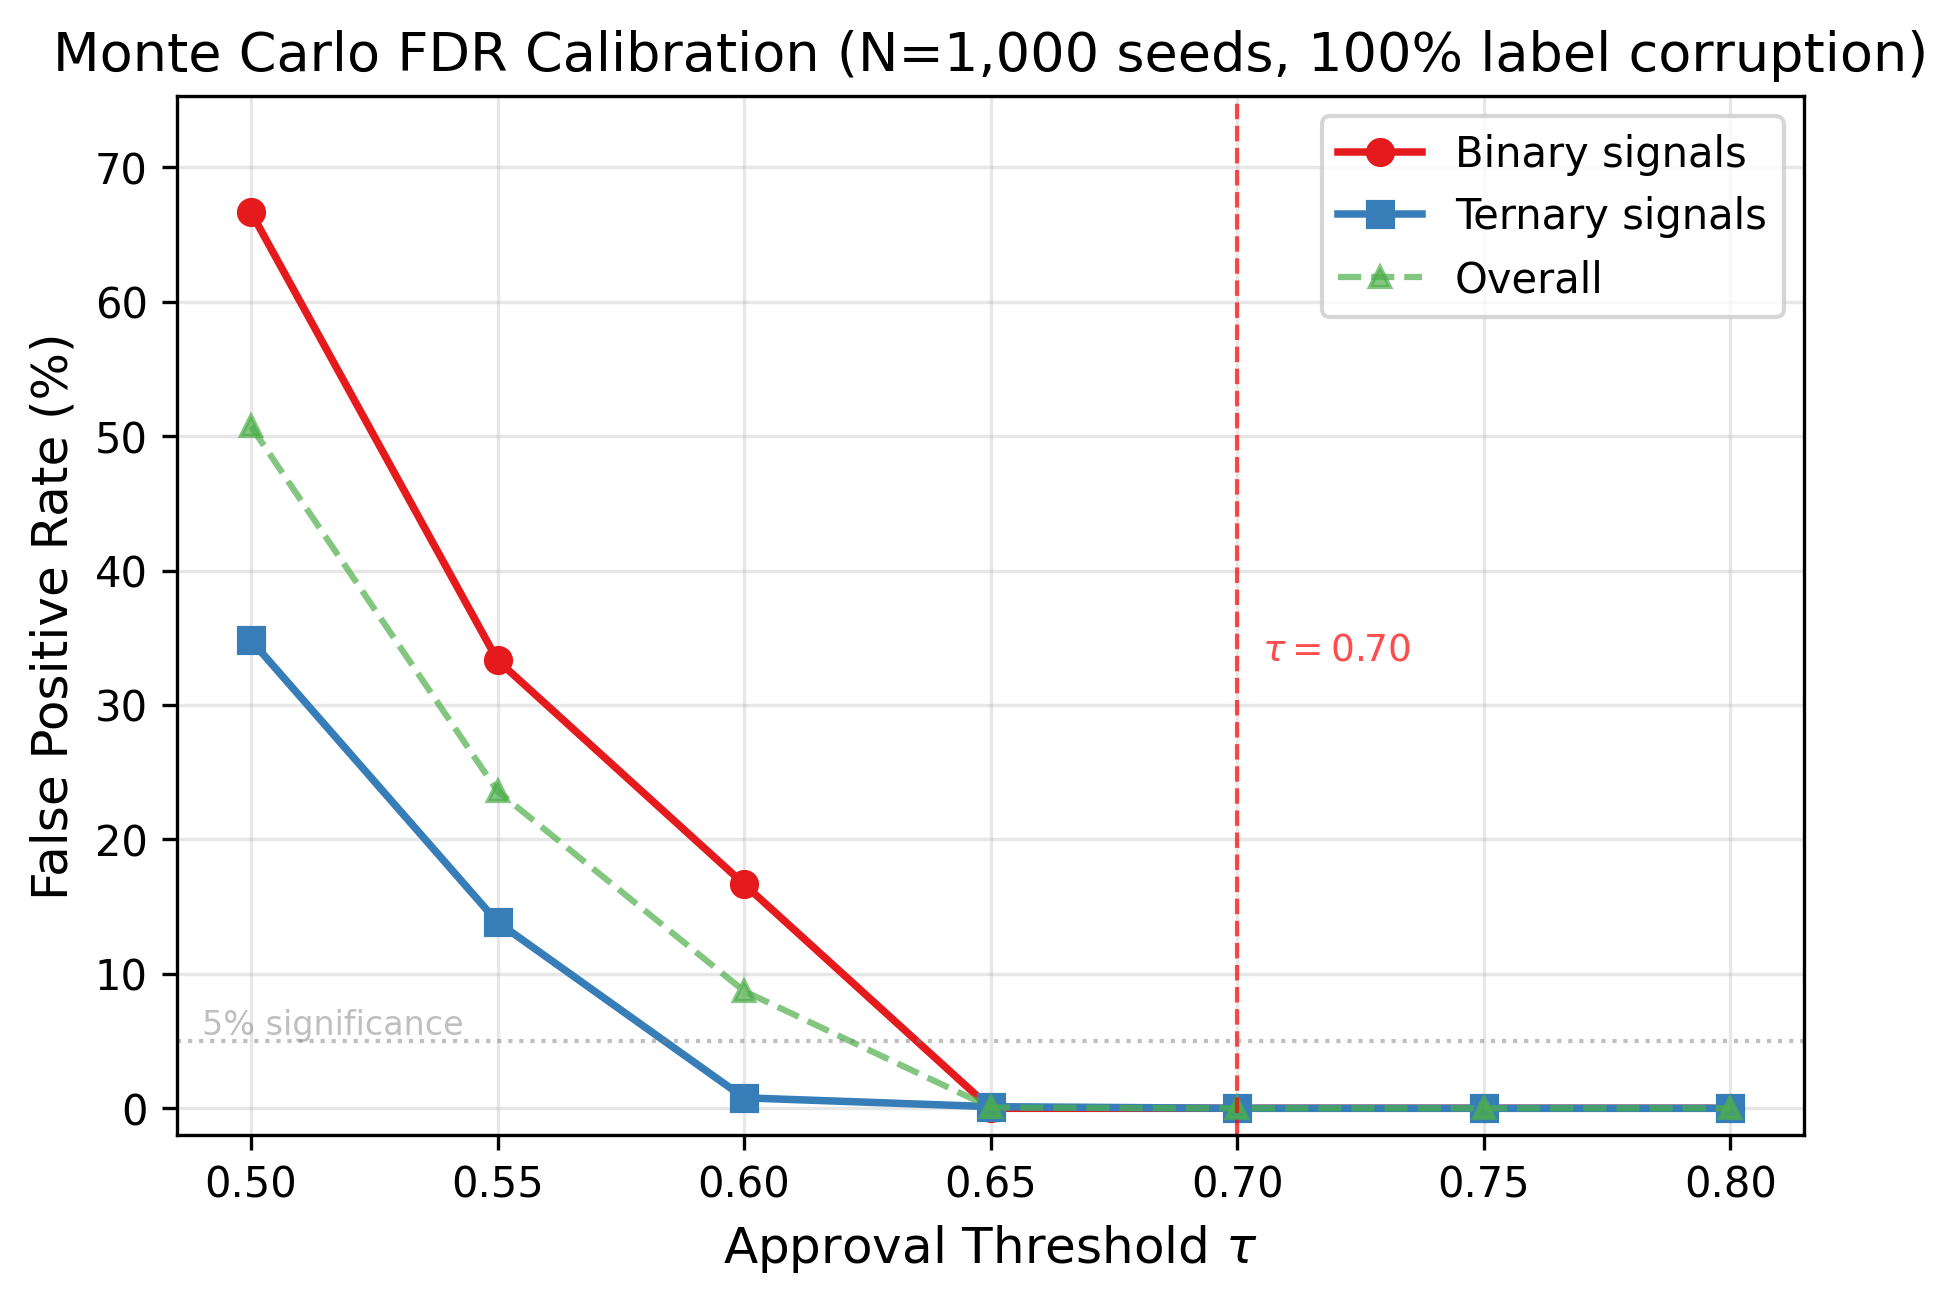
\includegraphics[width=0.85\textwidth]{figures/fig_fpr_curve.pdf}
\caption{False positive rate as a function of approval threshold $\tau$ under 100\% label corruption ($N=1{,}000$ Monte Carlo seeds). Binary signals have higher baseline FPR due to 50\% accidental label agreement versus 33\% for ternary. At $\tau \geq 0.70$, zero false positives are observed for both signal types.}
\label{fig:fpr}
\end{figure}


% ============================================================
\section{Discussion}
\label{sec:discussion}

\subsection{The Value of an Honest Negative Result}

The central empirical finding is positive DSR significance paired with non-significant Ledoit--Wolf tests against buy-and-hold. This combination may appear paradoxical, but it is informative. The DSR confirms that the approved signals capture genuine predictive structure after correcting for multiple testing ($N=12$). The Ledoit--Wolf test indicates that this structure does not translate into benchmark-beating returns given the available sample and the strong 2023 equity rally. Taken together, these results demonstrate that the SCS framework produces transparent, falsifiable conclusions rather than the kind of inflated claims that plague the ML trading literature.

\subsection{Robustness Is Not Performance}

SCS-A measures \emph{in-sample robustness}, not OOS alpha. The binding constraint is inter-model consensus: the 7 borderline groups have $S_{\text{model}}$ $\leq 0.36$. The best OOS performer among forced-through groups may not be among the 5 approved groups (SCS-A\,$<$\,0.70), demonstrating that SCS-A filters for robustness, not magnitude. This is confirmed quantitatively: the Spearman correlation between SCS-A and mean OOS Sharpe (across three windows) is $\rho = -0.405$ ($p = 0.32$, $N = 8$ pass-all groups), and using W3 alone yields $\rho = 0.119$ ($p = 0.78$). SCS-A is a \emph{filter}---it removes noise---but not a \emph{ranker}---higher scores do not predict higher returns. This is by design: a framework that guarantees high OOS returns would itself be an alpha source---an impossibility absent genuine predictive content.

\subsection{Addressing Known Pitfalls}

The pipeline addresses each of the validation gaps identified in the ML trading literature: temporal leakage (25-day embargo enforced by automated tests), multiple testing (DSR correction for $N=12$ trials), backtest multiplicity (single standardized engine), incomplete inference (four complementary statistical tests at Phase~C), and in-sample overfitting (three-phase temporal separation with go/no-go gates). The performance-weighted consensus measure, multi-window OOS testing, and FDR calibration strengthen the framework on the three specific dimensions where naive validation approaches are weakest.

\subsection{SCS Component Analysis}

The most discriminating SCS-A component is $S_{\text{model}}$ (mean\,=\,0.21, range 0.00--0.48), which is the primary driver of the 5/12 approval rate. Three groups---15d ternary, 10d ternary, and 3d ternary---receive $S_{\text{model}} = 0.00$ because their Kish effective $N < 5$, meaning that performance-weighted consensus collapses entirely when most model--asset conditions produce near-zero or negative returns. Among the 12 groups, $S_{\text{asset}}$ ranges from 0.40 to 0.86 (2.1$\times$ variation) while $S_{\text{seed}}$ ranges from 0.92 to 0.97 (1.05$\times$ variation). $S_{\text{time}}$ is uniformly high (mean\,=\,0.90, range 0.77--0.98), indicating that the 2010--2013 discovery window provides strong temporal consistency across all horizons. Cross-model agreement ($S_{\text{model}}$) and cross-asset generalization ($S_{\text{asset}}$) are the binding constraints for ML trading signals in this environment.

\textbf{Diagnostic: effect of performance weighting.} To isolate the impact of the weighting scheme, we recompute $S_{\text{model}}$ with uniform weights (standard Spearman, no profitability conditioning). The unweighted scores are substantially higher: for instance, 5d binary rises from 0.48 to 0.75, 10d binary from 0.38 to 0.78, and the borderline 20d binary from 0.12 to 0.81. Models agree on the \emph{rank ordering} of conditions overall, but they disagree on which \emph{profitable} conditions are best. Kish $N_{\text{eff}}$ reveals the mechanism: 5d binary retains 44\% of its 81 conditions as effective observations, while 20d binary retains only 18\%, indicating that a small number of high-weight conditions dominate the weighted consensus. The performance weighting thus acts as an intentional severity filter---it surfaces the fragility that an unweighted consensus measure would mask.

The walk-forward score's most informative component is $S_{\text{cost}}$, spanning 0.00 (3d ternary) to 0.96 (20d binary). Longer-horizon strategies trade less frequently and therefore absorb cost shocks more readily---an economically intuitive gradient that the SCS-B decomposition makes explicit.

\subsection{Discovery Window Sensitivity}

The same framework with identical hyperparameters ($\tau=0.70$, 12 signal groups, 3 models, 5 seeds) produces different results depending on the discovery window: the 2010--2013 window approves 5/12 groups with mean SCS-A of 0.68, whereas a 2015--2018 window approves 3/12 with mean SCS-A of 0.74 (Table~\ref{tab:window_contrast}). This is expected: SCS-A scores reflect the \emph{discoverability} of signals in the training data, not an absolute quality measure. Practitioners should not compare SCS-A scores across windows and should consider running the framework on multiple discovery periods.

\textbf{Choice of primary discovery window.} The 2010--2013 window was selected over 2015--2018 for three reasons: (i)~it spans the post-GFC recovery, capturing diverse market regimes (low-volatility recovery in 2010--2011, European debt crisis in 2011--2012, and the early QE-driven bull in 2013) that stress-test signal robustness more rigorously than the low-volatility expansion of 2015--2018; (ii)~with discovery ending in 2013, the walk-forward period 2014--2022 provides 9 years spanning multiple regimes (including the COVID crash) and 6 annual expanding folds, compared to 6 years and 3 folds with 2015--2018 discovery ending before 2019; (iii)~the longer walk-forward period produces better-calibrated $S_{\text{time}}^{(B)}$ scores in Phase~B and enables the three non-overlapping OOS test years (2023, 2024, 2025) that form the multi-window analysis. Both windows are 4 years in duration; the advantage of 2010--2013 lies in the \emph{downstream} validation capacity it affords.

\subsection{Limitations}

\textbf{$S_{\text{model}}$ design choice.} This paper adopts a performance-weighted Spearman formulation for $S_{\text{model}}$ that conditions inter-model consensus on profitability, guarded by a Kish effective-$N$ threshold. An alternative---counting statistically significant pairwise correlations without conditioning on profitability---is simpler but may overstate consensus when models agree on unprofitable conditions. Both formulations yield substantively identical conclusions when applied to the same 12-group search space: a small minority of signals pass, approved signals are statistically real but do not beat buy-and-hold, and the framework correctly rejects noise under corruption and FDR testing. The performance-weighted variant is adopted here as the stricter and recommended default for studies where consensus conditional on profitability is the relevant criterion.

\begin{enumerate}
  \item \textbf{Regime variation}: The multi-window extension (Section~\ref{sec:multiwindow}) shows that approved signals remain profitable across all three OOS years (2023--2025) but with substantial Sharpe ratio variation ($\sigma_{\text{SR}}$ up to 0.73). The framework certifies that signals have robust in-sample evidence, but it does not guarantee uniform performance across all regimes. Practitioners should combine SCS-approved signals with regime-detection or position-sizing overlays to manage drawdown risk. Additionally, the three windows differ in Phase~B training history length and fold count (W1: 2 folds over 4 years; W2/W3: 3 folds over 5--6 years), so cross-window differences partially confound regime effects with training-set size. A fully controlled comparison would require equal-length Phase~B windows, at the cost of wasting available data.
  \item \textbf{Discovery window sensitivity}: SCS-A is sensitive to the discovery window. The same framework with $\tau=0.70$ approves 5/12 groups in the 2010--2013 window but only 3/12 in a 2015--2018 window (Table~\ref{tab:window_contrast}). Practitioners must carefully select the discovery period and consider running the framework across multiple windows to assess stability.
  \item \textbf{Weak Spearman correlation}: Using one observation per signal group (mean OOS Sharpe across three windows, $N=8$ pass-all groups), the Spearman correlation with SCS-A is $\rho=-0.405$ ($p=0.32$); using W3 alone, $\rho=0.119$ ($p=0.78$). SCS-A is a robustness filter, not a performance predictor---higher SCS-A does not imply higher OOS returns.
  \item \textbf{Feature set}: The 11 technical indicators are deliberately parsimonious. Incorporating fundamental, sentiment, or alternative data sources could strengthen the signals while the same validation infrastructure applies unchanged.
  \item \textbf{Universe}: 27 US large-cap securities represents a limited, survivorship-biased universe (selected from current S\&P~500 membership and filtered for data availability back to 2010). When we extend the pipeline to a broader 159-ticker universe covering current S\&P\,500 members with sufficient data history, the SCS framework rejects all 12 signal groups (0/12 approved), confirming that survivorship-biased stock selection inflates in-sample robustness scores \citep{elton1996survivorship}. Extension to international markets, small caps, or other asset classes would test generalizability. The survivorship bias likely inflates OOS returns relative to a universe defined ex ante; the expanded-universe experiment quantifies this effect.
  \item \textbf{Threshold calibration}: With the 2010--2013 window, $\tau=0.70$ is the binding constraint (5/12 pass). However, the threshold's discriminating power depends on the signal environment: in future applications with different feature sets or universes, the cliff may shift. Practitioners should assess the threshold's position relative to the SCS-A distribution before deploying, and consider using the more conservative FDR-calibrated threshold ($\tau=0.75$, which also yields zero observed false positives in our calibration sample) as an alternative.
  \item \textbf{Computational cost}: The Phase~A grid requires $>$14,000 model fits. Although parallelizable, this scales poorly to higher-dimensional feature or hyperparameter spaces. Bayesian optimization could reduce the search while preserving the multi-dimensional validation structure.
  \item \textbf{Theoretical foundation}: As noted in Section~\ref{sec:interpretation}, SCS is a practitioner-oriented composite score with a robustness interpretation, not a formal statistical test. The Monte Carlo FDR calibration (Section~\ref{sec:fdr}) provides empirical false positive rates under the null, but a fully rigorous characterization---converting each sub-score to a calibrated $p$-value and combining via Fisher's method---would place SCS on firmer theoretical ground and is the subject of planned follow-up work.
  \item \textbf{Probability of Backtest Overfitting}: The PBO statistic \citep{bailey2017probability} computed with $S=6$ folds and $C(6,2)=15$ paths is 0.80, indicating that the single best IS strategy frequently underperforms the OOS median. This is expected: SCS replaces single-criterion IS ranking with multi-dimensional filtering. With only 15 combinatorial paths (below the $\geq$16 recommended by Bailey et al.), the PBO estimate has limited precision; the Monte Carlo FDR calibration (zero observed false positives at $\tau \geq 0.70$ over 12{,}000 null trials) provides a stronger overfitting control.
  \item \textbf{No live trading validation}: All results are from historical backtests. Slippage, market impact, and execution uncertainty may degrade live performance beyond what the 5~bps cost assumption captures, particularly for the higher-frequency 3d and 5d strategies.
  \item \textbf{Power analysis sample size}: Oracle injection uses $N=50$ seeds per noise level. At 96\% observed power (48/50), the Clopper--Pearson 95\% CI is approximately $[86\%, 100\%]$. Larger seed counts would tighten this bound.
  \item \textbf{Signal decay}: The declining average Sharpe from W1 (+1.07) through W3 (+0.60) is consistent with either regime variation or post-discovery signal decay \citep{mclean2016does}. Three windows are insufficient to distinguish these explanations; longer-horizon studies with additional OOS years would be needed to test for a secular trend.
\end{enumerate}


% ============================================================
\section{Conclusion}
\label{sec:conclusion}

This paper proposes the Signal Credibility Score (SCS), a multi-phase validation framework for machine learning trading signals that combines five robustness dimensions---temporal consistency, cross-asset generalization, inter-model consensus, seed stability, and trade distribution quality---into a composite go/no-go gate. The framework features a performance-weighted consensus measure that conditions inter-model agreement on profitability, multi-window out-of-sample testing across distinct market regimes, and Monte Carlo false discovery rate calibration with oracle-based power analysis. Applied to 12 signal groups (6 horizons $\times$ 2 labeling schemes) over 27 US equities, with discovery on 2010--2013 data, a primary walk-forward stage over 2014--2022, and complementary non-overlapping OOS evaluations over 2023--2025, the framework:

\begin{itemize}
  \item Identifies 5 of 12 groups as SCS-A-approved (SCS-A\,$\geq$\,0.70), with the $S_{\text{model}}$ component (scores 0.00--0.48) serving as the binding constraint by conditioning inter-model agreement on profitability (Figure~\ref{fig:heatmap}).
  \item Validates all 5 through expanding walk-forward analysis (6 folds, 2014--2022) under dual cost scenarios.
  \item Confirms regime robustness more cautiously: under the strict pipeline, 4 of 5 approved groups pass Phase~B across three non-overlapping OOS evaluations (2023--2025) and record positive Sharpe in every window. A complementary forced-through diagnostic evaluation shows 8 of 12 groups averaging Sharpe\,=\,+1.07, +1.39, and +0.60 respectively, though with substantial cross-window variation ($\sigma_{\text{SR}}$ up to 0.73).
  \item Achieves zero observed false positives at $\tau \geq 0.70$ ($0/12{,}000$ null trials; 95\% CI: $[0, 0.03\%]$) while oracle injection yields 96--100\% observed detection power across the tested noise levels (Figure~\ref{fig:power}, Figure~\ref{fig:fpr}).
\end{itemize}

The performance-weighted consensus measure, multi-window OOS testing, and FDR calibration address three critical gaps in the ML trading validation literature---consensus inflation, single-window fragility, and uncalibrated false positive rates---while maintaining the framework's core properties: pre-specified gates, multi-dimensional screening, and reproducible statistical evidence.

The paper's central contribution is not the discovery of profitable signals---the approved strategies do not beat buy-and-hold---but rather a replicable validation protocol that \emph{honestly separates robust signals from noise} and reports transparent, falsifiable conclusions. In an era where most ML trading studies overstate their findings, a framework that rejects 58\% of candidates and openly quantifies what remains is, we argue, more valuable than one that maximizes reported returns.

The complete pipeline (approximately 5{,}800 lines of Python across 37 modules, 42 automated tests, 14,580 model runs, 135,000+ trades) is open-source and fully reproducible.


% ============================================================
\section*{Code Availability}

The complete implementation---including the performance-weighted $S_{\text{model}}$, multi-window OOS pipeline, FDR simulation, and power analysis---is available at \url{https://github.com/HamzaKhan2002/scs-framework}. The repository contains approximately 5{,}800 lines of Python across 37 modules, 42 automated tests, and all experiment result files needed to reproduce every number in this paper.


% ============================================================
\section*{Author Contributions (CRediT)}

\textbf{Hamza Khan:} Conceptualization (lead), Methodology (lead), Software (lead), Validation, Formal Analysis, Investigation, Data Curation, Writing---Original Draft, Writing---Review \& Editing, Visualization.
\textbf{Alexandre Danoffre:} Conceptualization (supporting), Methodology (supporting), Software (supporting---initial framework prototype).

A.~Danoffre developed the initial prototype of the SCS framework as part of a joint final-year engineering project at ECE Paris. H.~Khan redesigned the scoring methodology (including the performance-weighted $S_{\text{model}}$, Kish guard, and multi-window extension), implemented the full pipeline, conducted all experiments, wrote the manuscript, and is the corresponding author.


% ============================================================
\section*{Acknowledgments}

This paper originates from a final-year engineering project (\textit{Projet de Fin d'\'{E}tudes}) at ECE Paris. We thank the ECE Paris engineering faculty for institutional support. Computational experiments were performed on cloud GPU infrastructure (RunPod). The authors declare no conflicts of interest and received no external funding for this research.


% ============================================================

\begin{thebibliography}{30}

\bibitem[Arnott et~al.(2019)]{arnott2019backtesting}
Arnott, R.~D., Harvey, C.~R., and Markowitz, H. (2019).
\newblock A backtesting protocol in the era of machine learning.
\newblock \emph{The Journal of Financial Data Science}, 1(1):64--74.

\bibitem[Bailey and L{\'o}pez~de~Prado(2014)]{bailey2014deflated}
Bailey, D.~H. and L{\'o}pez~de~Prado, M. (2014).
\newblock The deflated Sharpe ratio: Correcting for selection bias, backtest
  overfitting, and non-normality.
\newblock \emph{The Journal of Portfolio Management}, 40(5):94--107.

\bibitem[Bailey et~al.(2017)]{bailey2017probability}
Bailey, D.~H., Borwein, J.~M., L{\'o}pez~de~Prado, M., and Zhu, Q.~J. (2017).
\newblock The probability of backtest overfitting.
\newblock \emph{Journal of Computational Finance}, 20(4):39--69.

\bibitem[Ben-Tal et~al.(2009)]{ben2009robust}
Ben-Tal, A., El~Ghaoui, L., and Nemirovski, A. (2009).
\newblock \emph{Robust Optimization}.
\newblock Princeton University Press.

\bibitem[Benjamini and Hochberg(1995)]{benjamini1995controlling}
Benjamini, Y. and Hochberg, Y. (1995).
\newblock Controlling the false discovery rate: A practical and powerful approach to multiple testing.
\newblock \emph{Journal of the Royal Statistical Society: Series B}, 57(1):289--300.

\bibitem[Cawley and Talbot(2010)]{cawley2010overfitting}
Cawley, G.~C. and Talbot, N.~L.~C. (2010).
\newblock On over-fitting in model selection and subsequent selection bias in performance evaluation.
\newblock \emph{Journal of Machine Learning Research}, 11:2079--2107.

\bibitem[Chen and Guestrin(2016)]{chen2016xgboost}
Chen, T. and Guestrin, C. (2016).
\newblock {XGBoost}: A scalable tree boosting system.
\newblock In \emph{Proceedings of the 22nd ACM SIGKDD Conference}, pp.~785--794.

\bibitem[Chen and Zimmermann(2022)]{chen2022open}
Chen, A.~Y. and Zimmermann, T. (2022).
\newblock Open source cross-sectional asset pricing.
\newblock \emph{Critical Finance Review}, 11(2):207--264.

\bibitem[Chordia et~al.(2020)]{chordia2020anomalies}
Chordia, T., Goyal, A., and Saretto, A. (2020).
\newblock Anomalies and false rejections.
\newblock \emph{The Review of Financial Studies}, 33(5):2134--2179.

\bibitem[Duchi and Namkoong(2021)]{duchi2021learning}
Duchi, J.~C. and Namkoong, H. (2021).
\newblock Learning models with uniform performance via distributionally robust optimization.
\newblock \emph{The Annals of Statistics}, 49(3):1378--1406.

\bibitem[Elton et~al.(1996)]{elton1996survivorship}
Elton, E.~J., Gruber, M.~J., and Blake, C.~R. (1996).
\newblock Survivorship bias and mutual fund performance.
\newblock \emph{The Review of Financial Studies}, 9(4):1097--1120.

\bibitem[Fischer and Krauss(2018)]{fischer2018deep}
Fischer, T. and Krauss, C. (2018).
\newblock Deep learning with long short-term memory networks for financial
  market predictions.
\newblock \emph{European Journal of Operational Research}, 270(2):654--669.

\bibitem[Gu et~al.(2020)]{gu2020empirical}
Gu, S., Kelly, B., and Xiu, D. (2020).
\newblock Empirical asset pricing via machine learning.
\newblock \emph{The Review of Financial Studies}, 33(5):2223--2273.

\bibitem[Harvey and Liu(2015)]{harvey2015backtesting}
Harvey, C.~R. and Liu, Y. (2015).
\newblock Backtesting.
\newblock \emph{The Journal of Portfolio Management}, 42(1):13--28.

\bibitem[Harvey and Liu(2020)]{harvey2020false}
Harvey, C.~R. and Liu, Y. (2020).
\newblock False (and missed) discoveries in financial economics.
\newblock \emph{The Journal of Finance}, 75(5):2503--2553.

\bibitem[Harvey et~al.(2016)]{harvey2016cross}
Harvey, C.~R., Liu, Y., and Zhu, H. (2016).
\newblock \ldots and the cross-section of expected returns.
\newblock \emph{The Review of Financial Studies}, 29(1):5--68.

\bibitem[Ke et~al.(2017)]{ke2017lightgbm}
Ke, G., Meng, Q., Finley, T., et~al. (2017).
\newblock {LightGBM}: A highly efficient gradient boosting decision tree.
\newblock In \emph{Advances in Neural Information Processing Systems}, 30:3146--3154.


\bibitem[Kish(1965)]{kish1965survey}
Kish, L. (1965).
\newblock \emph{Survey Sampling}.
\newblock John Wiley \& Sons.

\bibitem[Krauss et~al.(2017)]{krauss2017deep}
Krauss, C., Do, X.~A., and Huck, N. (2017).
\newblock Deep neural networks, gradient-boosted trees, random forests:
  Statistical arbitrage on the S\&P\,500.
\newblock \emph{European Journal of Operational Research}, 259(2):689--702.

\bibitem[Ledoit and Wolf(2008)]{ledoit2008robust}
Ledoit, O. and Wolf, M. (2008).
\newblock Robust performance hypothesis testing with the Sharpe ratio.
\newblock \emph{Journal of Empirical Finance}, 15(5):850--859.

\bibitem[L{\'o}pez~de~Prado(2018)]{lopez2018advances}
L{\'o}pez~de~Prado, M. (2018).
\newblock \emph{Advances in Financial Machine Learning}.
\newblock John Wiley \& Sons.

\bibitem[McLean and Pontiff(2016)]{mclean2016does}
McLean, R.~D. and Pontiff, J. (2016).
\newblock Does academic research destroy stock return predictability?
\newblock \emph{The Journal of Finance}, 71(1):5--32.

\bibitem[Pardo(2008)]{pardo2008evaluation}
Pardo, R. (2008).
\newblock \emph{The Evaluation and Optimization of Trading Strategies}.
\newblock John Wiley \& Sons, 2nd edition.

\bibitem[Politis and Romano(1994)]{politis1994stationary}
Politis, D.~N. and Romano, J.~P. (1994).
\newblock The stationary bootstrap.
\newblock \emph{Journal of the American Statistical Association}, 89(428):1303--1313.

\bibitem[Sharpe(1994)]{sharpe1994sharpe}
Sharpe, W.~F. (1994).
\newblock The Sharpe ratio.
\newblock \emph{The Journal of Portfolio Management}, 21(1):49--58.

\bibitem[White(2000)]{white2000reality}
White, H. (2000).
\newblock A reality check for data snooping.
\newblock \emph{Econometrica}, 68(5):1097--1126.

\end{thebibliography}


% ============================================================
\appendix
\section{SCS-A Component Formulas}
\label{app:scs_a}

The robustness score function shared by $S_{\text{time}}$ and $S_{\text{asset}}$ is:

\begin{equation}
  R(\mathbf{v}) = 0.30 \cdot \underbrace{\frac{|\{v_i > 0\}|}{n}}_{\text{sign ratio}}
  + 0.20 \cdot \underbrace{e^{-\text{CV}(\mathbf{v})}}_{\text{stability}}
  + 0.25 \cdot \underbrace{\min(1, |\bar{v}|/0.5)}_{\text{magnitude}}
  + 0.25 \cdot \underbrace{f(\min(\mathbf{v}))}_{\text{worst case}}
\end{equation}

where $\text{CV} = \sigma / (|\mu| + \epsilon)$ and:

\begin{equation}
  f(x) = \begin{cases}
    1.0 & \text{if } x > -0.5 \\
    \max(0, 1 + (x+0.5)/0.5) & \text{if } -1.0 < x \leq -0.5 \\
    0.0 & \text{if } x \leq -1.0
  \end{cases}
\end{equation}

\subsection*{$S_{\text{seed}}$: Stochastic Seed Stability}

$S_{\text{seed}}$ measures whether performance is stable across random initialization seeds. Let $\bar{v}_s$ be the mean Sharpe ratio of seed~$s$ across all conditions. The score combines:

\begin{equation}
  S_{\text{seed}} = 0.40 \cdot \underbrace{\frac{|\{s : \bar{v}_s > 0\}|}{|\mathcal{S}|}}_{\text{sign ratio}}
  + 0.30 \cdot \underbrace{e^{-\text{CV}(\mathbf{\bar{v}})}}_{\text{stability}}
  + 0.30 \cdot \underbrace{e^{-\bar{\sigma}_r / |\mathcal{S}|}}_{\text{ranking stability}}
\end{equation}

where $\bar{\sigma}_r$ is the mean standard deviation of seed ranks across conditions. A hard gate caps $S_{\text{seed}} \leq 0.30$ if the sign ratio falls below~0.40.

\subsection*{$S_{\text{dist}}$: Trade-Level Distributional Quality}

$S_{\text{dist}}$ evaluates the statistical health of realized trade returns $\{r_1, \ldots, r_N\}$ pooled across all conditions:

\begin{equation}
  S_{\text{dist}} = 0.25 \cdot c_{\text{skew}} + 0.20 \cdot c_{\text{kurt}} + 0.35 \cdot c_{\text{win}} + 0.15 \cdot c_{\text{cv}} + 0.05 \cdot c_{\text{conc}}
\end{equation}

where $c_{\text{skew}}$ scores absolute skewness (1.0 if $|\gamma_1| \leq 5$), $c_{\text{kurt}}$ scores excess kurtosis (1.0 if $\kappa \leq 8$), $c_{\text{win}}$ scores the win ratio (1.0 if $\geq$45\%), $c_{\text{cv}}$ scores trade-size stability via the coefficient of variation of $|r_i|$, and $c_{\text{conc}}$ penalizes profit concentration in a few large trades. If $N < 20$, the score defaults to 0.30.

\subsection*{$S_{\text{model}}$: Performance-Weighted Inter-Model Consensus}

For each signal group $(H, L)$, we compute pairwise Spearman rank correlations across model types, weighted by condition-level profitability. Let $c = (\text{ticker}, \text{period})$ index a training condition and let $\text{SR}_{i,c}$ be the in-sample Sharpe ratio of model $i$ under condition $c$. The weight for condition $c$ is:

\begin{equation}
  w_c = \max\!\left(\max_i \text{SR}_{i,c},\; 0\right)
\end{equation}

This assigns zero weight to conditions where no model is profitable, focusing the consensus measurement on informative conditions. For each model pair $(i, j)$, the weighted Spearman correlation $\rho_{ij}^{(w)}$ is computed using these weights. The raw consensus score is:

\begin{equation}
  S_{\text{model}}^{\text{raw}} = \max\!\left(\bar{\rho}_w,\; 0\right), \quad \bar{\rho}_w = \frac{2}{M(M-1)} \sum_{i < j} \rho_{ij}^{(w)}
\end{equation}

where $M$ is the number of model types. A Kish effective-$N$ guard \citep{kish1965survey} ensures sufficient diversity of informative conditions:

\begin{equation}
  N_{\text{eff}} = \frac{\left(\sum_c w_c\right)^2}{\sum_c w_c^2}
\end{equation}

If $N_{\text{eff}} < 5$, weight concentration is too high (a few conditions dominate the consensus estimate) and $S_{\text{model}} = 0$. Otherwise, $S_{\text{model}} = S_{\text{model}}^{\text{raw}}$.


\section{Portfolio Backtest Mechanics}
\label{app:backtest}

The execution parameters introduced in Section~\ref{sec:execution} are operationalized as follows. Each trading day involves four steps:

\begin{enumerate}
  \item \textbf{Stop-loss / take-profit check.} Open positions are evaluated using the directional return from the entry price. A stop-loss triggers at $-5\%$ and a take-profit at $+8\%$.
  \item \textbf{Horizon exit.} Positions that have reached their planned holding period ($H$ trading days) are closed at the day's closing price.
  \item \textbf{New entries.} Tickers are ranked by predicted probability; only signals with $P \geq 0.55$ are eligible. Positions are opened subject to a maximum of 15 simultaneous positions and a per-ticker exposure cap of 12\% of equity.
  \item \textbf{Mark-to-market.} Equity is updated including unrealized P\&L on all open positions.
\end{enumerate}

\textbf{Entry-price convention and label mismatch.} Positions are entered at the \emph{closing price of the signal date} ($\text{Close}(t)$), whereas the labeling formula (Section~\ref{sec:methodology}) defines returns relative to $\text{Open}(t{+}1)$: $r_t(H) = \text{Close}(t{+}H) / \text{Open}(t{+}1) - 1$. This creates a systematic wedge---the overnight gap between $\text{Close}(t)$ and $\text{Open}(t{+}1)$---that slightly misaligns label returns and realized returns. The discrepancy is conservative on average (buying at the close when the label assumes the next open), but it constitutes an implementation shortfall that live execution would need to manage via limit orders near the close or at the open.

Transaction costs are fixed basis points on traded notional (5~bps baseline, 15~bps stress) with no market-impact or slippage model. The annualized Sharpe ratio is $\text{SR} = (\bar{r}_d / \sigma_d) \times \sqrt{252}$, computed from the daily equity curve.


\section{Complete SCS-A and SCS-B Results}
\label{app:full_results}

\begin{table}[H]
\centering
\caption{Phase A Hard Gate Summary}
\label{tab:rejection}
\begin{tabular}{lll}
\toprule
Signal Group & Mean Sharpe & Status \\
\midrule
\multicolumn{3}{l}{\textit{No groups rejected by hard gates in this run.}} \\
\multicolumn{3}{l}{\textit{All 12 groups have positive mean Sharpe and positive ratio $>$ 0.50.}} \\
\bottomrule
\end{tabular}
\end{table}


\end{document}
